The project described in this chapter was the second large project of my PhD and involved making significant changes to the PyCBC Live search. The changes to the PyCBC Live code were made by myself however to use these changes in the live search for gravitational waves another significant set of changes were required to implement the structural changes that define how PyCBC Live runs on the supercomputer infrastructure. Therefore this work has not currently been published, it is aimed to form part of the PyCBC Live fourth observing run methods paper. Significant contributions were made by Gareth Cabourn Davies and Max Trevor to enable these changes to be run in the second half of the fourth observing run.

\section{\label{sec:pycbclive-introduction}Introduction}

The PyCBC offline search is the most sensitive gravitational wave search pipeline~\cite{PyCBC:2016, PyCBC:2017, PyCBC_package:2021}. The PyCBC live search pipeline however, is lagging behind. In the third and first half of the fourth observing runs the GstLAL pipeline~\cite{GstLAL:2020} was the preferred event for X of the Y events whereas PyCBC live was only preferred in Z events. We want to improve the PyCBC live search to be of the same calibre as its offline counterpart and to do this we must look at the key differences between the two searches.

The offline search is capable of using information determine post-gravitational wave detection in its results and also has no limit on the amount of processing that can be done to find events. The live search in contract must detect these events with as little latency as possible and therefore cannot use post-event information and is also limited in its processing requirements due to computational cost introducing an untenable amount of lag to the search. Even with these two restrictions there are components to the offline search that can be adapted and incorporated into the live search. Including new components into the live search we will improve the sensitivity of the search, detecting more gravitational wave events with greater significance.

\section{\label{sec:pycbclive-ranking-stat}The Ranking Statistic}

SO UGLY REWRITE THE WHOLE THING

These additional components that we can take from the offline search and include in the live search come about in the ranking statistic that the searches use. The ranking statistic is the post-detection quantification of legitimacy of a gravitational wave detection and can be directly mapped to the false-alarm rate~\cite{PyCBC_global:2020}.

The PyCBC ranking statistic is constructed using separate contributions from single and coincidence detector information. The single detector ranking is calculated first and then coincidence information is incorporated to determine the final ranking statistic. 

The single detector ranking statistic components are as follows:
\paragraph{newsnr}

is the original matched filter SNR, $\rho$, with the signal consistency Allen $\chi^{2}$~\cite{Allen_Chi:2005} test applied to construct a new SNR value, $\hat{\rho}$.

\paragraph{sgveto}

is the inclusion of the sine-gaussian $\chi^{2}$ test in the computation of the new SNR value.

\paragraph{psdvar\_threshold}

includes the PSD variation measurement in the calculation of the new SNR. The \verb|threshold| applies a hard cut to the allowed $\chi^{2}$ and PSD variation values of $10.0$, where all triggers found with above this value will receive a new SNR of $1.0$.

The coincident detector ranking statistic components are:
\paragraph{dq}
includes a likelihood ratio correction made possible by estimating the relative noise trigger rates based on the data quality veto time series.

\paragraph{phasetd}
re-ranks the combined new SNR of the two detectors and re-weights them based on coincidence parameters. The weighting is determined by a PDF of time delays, phase differences and amplitude ratios between the two detector triggers. Some combinations of these coincidence parameters will be more likely therefore the triggers will be ranked depending on how likely the event was to occur.

\paragraph{exp\_fit\_fgbg}
uses an exponential model to describe the falloff of the noise distribution at higher SNRs. The statistic calculated the log noise coincidence rate for each template using the single detector trigger new SNR values.

\paragraph{kde}
applies a mass and spin dependent weighting factor determine using KDE statistic files. The likelihood ratio is multiplied by the ratio of signal KDE to template KDE over some parameters covering the bank.

\section{\label{sec:pycbclive-previous-stat}Ranking Statistic Used in O3}

The PyCBC Live ranking statistic used in the third and second half of the fourth observing run remained the same and takes the form:
%
\begin{minted}{python}
sngl-ranking = newsnr_sgveto
ranking-statistic = phasetd
\end{minted}
%
whereas the currently used PyCBC Offline ranking statistic is as follows:
%
\begin{minted}{python}
sngl-ranking = newsnr_sgveto_psdvar_threshold
ranking-statistic = dq_phasetd_exp_fit_fgbg_kde
\end{minted}
%
where it can be seen quite clearly that the PyCBC Live ranking statistic is missing many components that the offline statistic has. Namely the PSD variation in the single detector statistic, the data quality correction, exponential noise falloff model and the KDE weighting.

Of these missing components three of them depend on extra files being created to be used in the search where the PSD variation is the only one that doesn't. These extra files are difficult (but not impossible) for the live search to produce.

\section{\label{pycbclive-new-additions}Adding to the PyCBC Live Ranking Statistic}

As previously mentioned, to improve the PyCBC Live ranking statistic we can a include some of the offline components that we currently are not using. We have chosen to adapt and include the PSD variation in the single detector ranking statistic and the exponential noise falloff model to the coincident ranking statistic to improve the sensitivity of the PyCBC Live search.

The data quality likelihood ratio correction cannot be included in the live search. The flags themselves are produced as the data arrives and therefore the live search cannot produce a statistic file without introducing lag to the search.

With the exponential noise falloff model however, we are able to make the assumption that the noise distribution remains constant over a small period of time. Therefore if we estimate the noise falloff for a week before the search we would expect this to be descriptive of the proceeding week's noise distributions and therefore will still increase the sensitivity of the search.

We haven't considered including the KDE statistic in the live ranking statistic simply due to time constraints with having already chosen the other two statistic components to include. We assume however that this is possible and the creation and inclusion of these files in the live ranking statistic is possible and can be done in the future.

\subsection{\label{pycbclive-psd-var}PSD Variation}

% What is a PSD and how do we measure it
A power spectral density (PSD) describes a signal's power at each discrete frequency. The PSD of the gravitational wave data is used in the matched filter equation,
%
% Matched Filter Equations
%
to calculate the SNR of a trigger and a PSD which doesn't accurately describe the noise profile of the data will lead to a miss-estimation in the SNR calculation. The offline search empirically measures the PSD of the gravitational wave data being analysed using Welch's method, however, instead of using a mean average of the overlapping PSDs a median average it used to remove the effect of short duration glitches in the data.

% What is the problem of non-stationary noise
This PSD is used for very long search segments ($512$ seconds) and while the effects of short duration glitches have been mitigated with the median average method we still suffer from the effects of non-stationary noise. Non-stationary noise is that which originates from instrumental noise such as seismic noise, thermal noise and quantum noise and cannot be mitigated except through detector improvements. This non-stationary noise will change the noise profile over the period of the search segment, meaning our PSD will be inaccurate at different times. Furthermore, there are different forms of non-stationary noise, we can distinguish between noise which has a constant mean and variance and that which have either a non-stationary mean or variance. Examples of these are shown in figure~ADD~\cite{Mozzon_Thesis:2023},
%
% Figure 4.1 Simone's Thesis
%

% What is PSD Variation
The mismatch between the estimated and actual PSD of the data will have the effect of underestimating and overestimating the noise at different times in our search segment. We are able to track the sources of the non-stationary noise in some cases, for example, when the source of the non-stationary noise is a period of increased seismic activity this will be identified by the seismometer auxiliary channels and can there be subtracted from the gravitational wave data. This isn't true for all noise however, some non-stationary noise has no immediately identifiable source and we are unable to make the subtraction.

Therefore we must track the difference between the estimated PSD and the actual PSD using the PSD variation statistic~\cite{PSD_var:2020}. The PSD variation statistic models the relationship between the estimated PSD and the actual PSD as follows,
%
\begin{equation}
    S_{A} = \nu_{s} S_{E}, 
\end{equation}
%
where $S_{A}$ is the actual PSD, $S_{E}$ is the estimated PSD and $\nu_{s}$ is a frequency independent parameter. The PSD variation is defined as the time series which tracks $\nu_{s}$ and computing $\nu(t)_{s}$ will deliver the PSD variation statistic that we can use to calculate the different between the actual and estimated PSDs at all times in our search data.

In the offline search $\nu(t)_{s}$ is calculated using an approximate expression for a typical CBC template, $|h(f)| \propto f^{\frac{-7}{6}}$, and the estimated PSD are used to construct a filter,
%
\begin{equation}
    F = \frac{|h(f)|}{S_{E}} ,
\end{equation}
%
which is band-passed between $20$Hz and $480$Hz, smoothed with a Hann window and combined with the data to produce an equation for the PSD variation time series,
%
\begin{equation}
    \nu(t)_{s} \equiv N \langle\rho^{2}\rangle(t), 
\end{equation}
%
where $N$ is a constant such that the expectation value of $\nu_{s}$ in Gaussian noise is $1$ and $\langle\rho^{2}\rangle$ is the SNR variance. This produces our required PSD variation time series that can then be applied to the offline search as part of the single detector ranking statistic where triggers are assigned the PSD variation value at trigger time which is used to re-weight the SNR before any signal consistency tests are applied,
%
\begin{equation}
    \rho^{2} = \frac{\rho^{2}}{\sqrt{\nu_{s}}} .
\end{equation}

% PSD Variation in Live

% How does the live search differ from the offline search?
The live search maintains a data ring buffer of $512$ seconds, rolling the newest eight seconds of data on as the older eight seconds are rolled off. The live search can be operating for potentially weeks at a time thereby requiring a dynamic PSD which can update during runtime. The initial PSD is estimated using Welch's method with a median average and is first created when enough data has been accumulated after starting the search. Every search stride (eight seconds) a new PSD is estimated and compared to the current search PSD. The comparison is made using the neutron star binary distance the distance a binary neutron star system of equal $1.4 M_{\odot}$ masses would need to be from our detectors to be observed with an SNR of $8.0$. If the new PSD's BNS distance differs from the current PSD's BNS distance by $\pm1\%$ the new PSD replaces the old one. If the new PSD is within the threshold, the new PSD is discarded and the search continues with the initial PSD. 

% How is the PSD variation calculated in Live
The live search does not need to calculate the PSD variation time series for the entire data ring buffer, new triggers are only ever found in the latest segment stride and therefore this is the only period of time for which the different between the estimated and the actual PSD matters. To calculate the PSD variation values we need to track the estimated PSD being used by each detector and create a new filter (equation~ADD) for each detector which is also updated every time the estimated PSD is updated. The filters are then convolved with the latest eight seconds in the data ring buffers, the mean square of the PSD variation time series is calculated every $0.25$ seconds to find outliers caused by short duration glitches. These outliers and then replaced with an average of the adjacent elements in the PSD variation time series and the time series is then further averaged every second to produce the final PSD variation time series. It is from this PSD variation time series that when a trigger is produced by the search, a PSD variation value is taken by interpolating between the two nearest whole seconds to the trigger time. This PSD variation value is then used in equation~ADD to reweight the SNR of the trigger.

\subsection{\label{pycbclive-template-fits}Modelling the Noise Falloff in Live}

% Introduce the need for modelling the noise falloff
Non-gaussian noise artefacts (glitches) can produce high SNR triggers, these are partially mitigated with the single detector ranking statistic signal consistency tests but there is still a long tail in the noise distribution that can be attributed to the effects of glitches.
%
% Figure of the noise falloff 
%
This noise falloff has historically been assumed to be gaussian in the PyCBC Live search and all templates are treated equally. There are a number of very common glitches that occur frequently in the data that can match more closely to some templates in the template bank and not others. An example of this is blip glitches~\cite{blips:2019} which resemble the gravitational wave signals of high mass binary black hole mergers, therefore the templates which describe these signals will trigger more regularly on these glitches with higher SNRs compared to other templates in the bank which do not look similar to any glitch class. Not only will the noise falloff no longer be gaussian, each template will have a different noise distribution so all templates should not be treated equally.

% Introduce the noise falloff model itself
PyCBC search triggers are only saved if they have an SNR above a set threshold normally $4.5$ for single detector triggers (meaning a network SNR threshold of $6.0$), therefore all triggers found with an SNR above this threshold make up the noise falloff. The noise falloff is modelled in PyCBC by taking all the triggers produced by a template and fitting an exponential model to the slope of the falloff giving the exponential fit factor, $\alpha$, and the rate of triggers found above another SNR threshold (normally $6.0$), $\mu$. This process is commonly called `template fitting' and the output parameters are called the `template fits' or simply `fits'.

PyCBC Offline searches through pre-defined chunks of IGWN data, which are all around one calendar week long. The search will matched filter the template bank and the data in one of these chunks and all triggers above the previously mentioned SNR threshold for each template are collected and saved. These triggers are then used for each template to calculate $\alpha$ and $\mu$ and these parameters are exported to data files which contain all of the template fits for the entire template bank for that chunk of data.
%
% Figure for the template fits
%
The template fits are then used to re-weight the ranking statistic of the coincident triggers. To understand how the template fits contributes to the ranking statistic we must first construct the ranking statistic which includes the noise falloff model. The optimal detection statistic can be given as,
%
\begin{equation}
    \Lambda_{opt}(\Vec{\kappa}) = \mu_{s} \frac{\Vec{r_{S}(\Vec{\kappa}})}{\Vec{r_{N}(\Vec{\kappa}})} ,
\end{equation}
where $\mu_{s}$ is the signal rate and is assumed to be constant, $\Vec{r_{S}(\Vec{\kappa}})$ is the signal event rate density and $\Vec{r_{N}(\Vec{\kappa}})$ is the noise event rate density. The signal and noise event rate densities are calculated and due to expected values spanning many orders of magnitude we take the logarithm of equation~ADD,
%
\begin{equation}
    R = \log(r_{s,i}) - \log(r_{n,i}) .
\end{equation}
The noise falloff model manifests in the noise event rate density. The noise event rate density is a combination of the single detector noise event rate densities,
%
\begin{equation}
    r_{n} = A_{N} \Pi_{d} r_{d}(\rho_{new}) ,
\label{eqn:pycbclive-comb-noise-rate}
\end{equation}
%
where $A_{N}$ is the `allowed area' for coincident noise events from two detectors, $A_{N\{12\}} = 2\tau_{12}$, where $\tau_{12}$ is the gravitational wave travel time window between detectors $1$ \& $2$ with a small allowance for timing error (currently $0.02$ seconds) and $r_{d}$ is the single detector noise event rate density for each detector $d$. The natural logarithm of this noise event rate density is taken to get the final combined log noise event rate,
%
\begin{equation}
    ln(r_{n}) = ln(A_{N}) +  \Sigma_{d} ln(r_{d}(\rho_{new})) .
\label{eqn:pycbclive-comb-log-noise-rate}
\end{equation}
%

The single detector noise event rate density is calculated using the product of the trigger rate above the template fitting SNR threshold, $\mu$, and the probability of the SNR given the template (including $\alpha$ and $\mu$) and noise,
%
\begin{equation}
    r_{d}(\rho_{new}; {\theta}; N) = \mu(\theta) p(\rho | \theta, N) ,
\label{eqn:pycbclive-single-noise-rate}
\end{equation}
%
where
%
\begin{equation}
    p(\rho_{new} | \theta, N) = \alpha(\theta) \exp\left(-\alpha(\theta)\left(\rho_{new} - \rho_{thresh}\right)\right)
\label{eqn:pycbclive-p-definition}
\end{equation}
%
thereby giving the single detector noise rate as,
%
\begin{equation}
    r_{d}(\rho_{new}; {\theta}, N) = \mu(\theta) \alpha(\theta) \exp\left(-\alpha(\theta)(\rho_{new} - \rho_{thresh})\right)
\label{eqn:pycbclive-single-noise-rate-full}
\end{equation}
%
and when the natural logarithm is taken we arrive at the complete single detector log noise event rate density,
%
\begin{equation}
    ln(r_{d}) = ln(\mu(\theta)) +  ln(\alpha(\theta)) - \alpha(\theta)(\rho_{new} - \rho_{thresh})
\label{eqn:pycbclive-single-log-noise-rate}
\end{equation}
%
for each detector, $d$.

% How is this put into PyCBC Live now
To generate template fits for a template bank the only requirements are the triggers for each template that you wish to fit an exponential function to. In the offline search we collect all of the triggers in a chunk and create the template fits to be used for that same chunk but PyCBC Live runs in low-latency and creating the template fits in real-time would be too computationally expensive. Therefore we make the choice to produce template fits from a set of triggers which will not contain the latest PyCBC Live triggers when used in the coincident ranking statistic. Every week the PyCBC Live search will collect and create the template fit files from the previous week of triggers, these will then be used for the next week and once again, after a week has passed the template fit files will be created again with the latest week's triggers. Unlike the offline search, the triggers themselves will not enter the noise distribution and we make the assumption that the noise distribution hasn't changed significantly and the fit files will still be representative by the end of the next week.


%%%% IAN COMMENT: WHY ARE YOU SHOWING THIS? COULD WE MAYBE COMPARE ONLINE VS OFFLINE FITS?
% %
% \begin{figure}
%   \centering
%   \begin{minipage}[t]{1.0\linewidth}
  
%     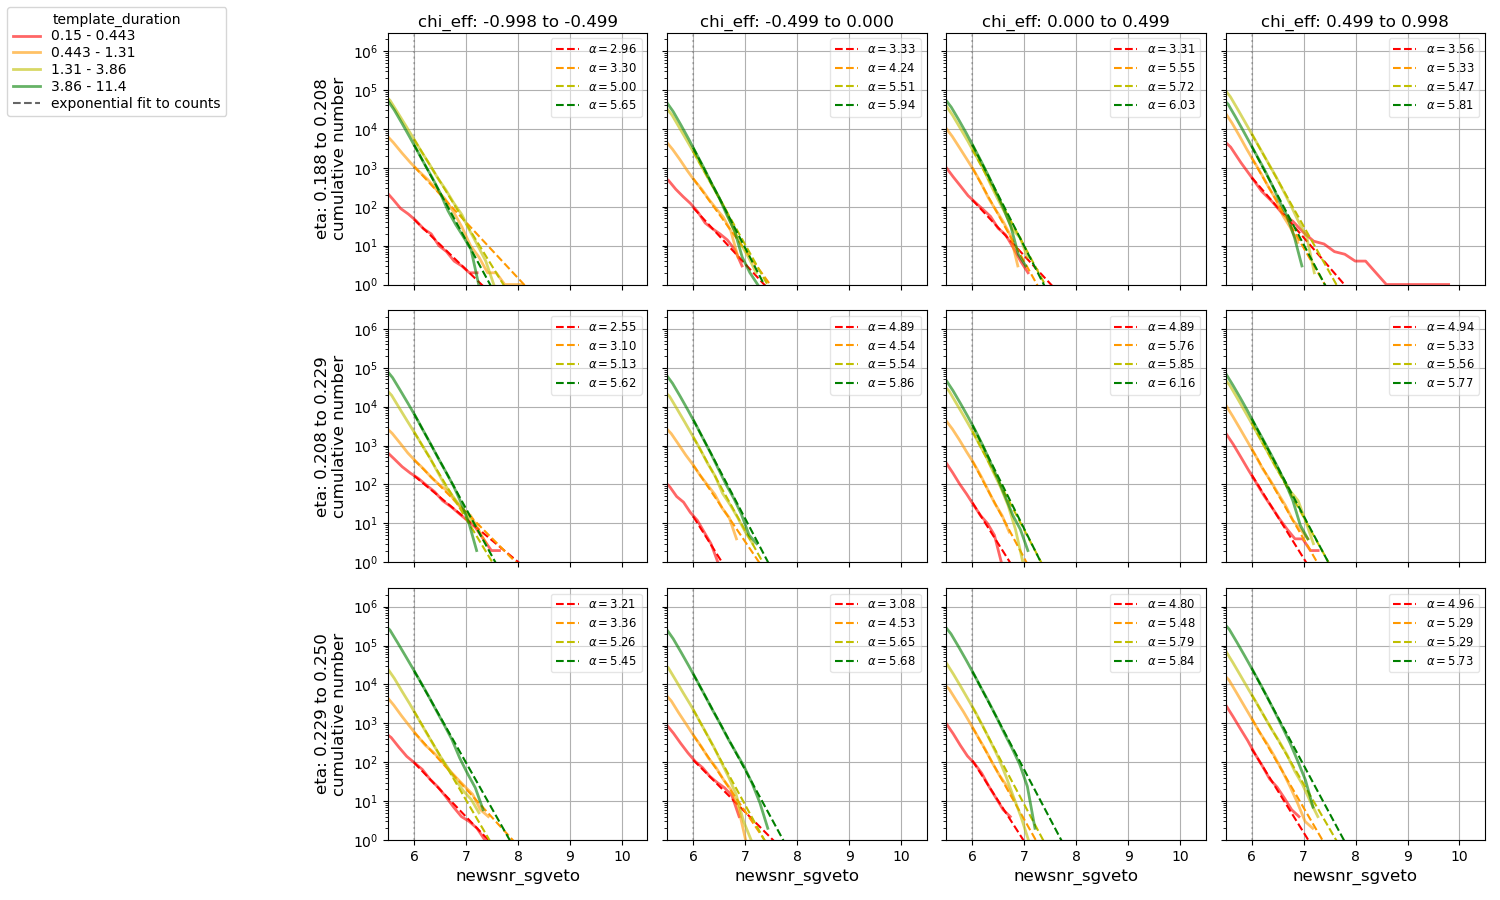
\includegraphics[width=1.0\textwidth]{images/5_pycbclive/H1-template_fits.png}
%     \label{fig:pycbclive-H1-fits}
  
%     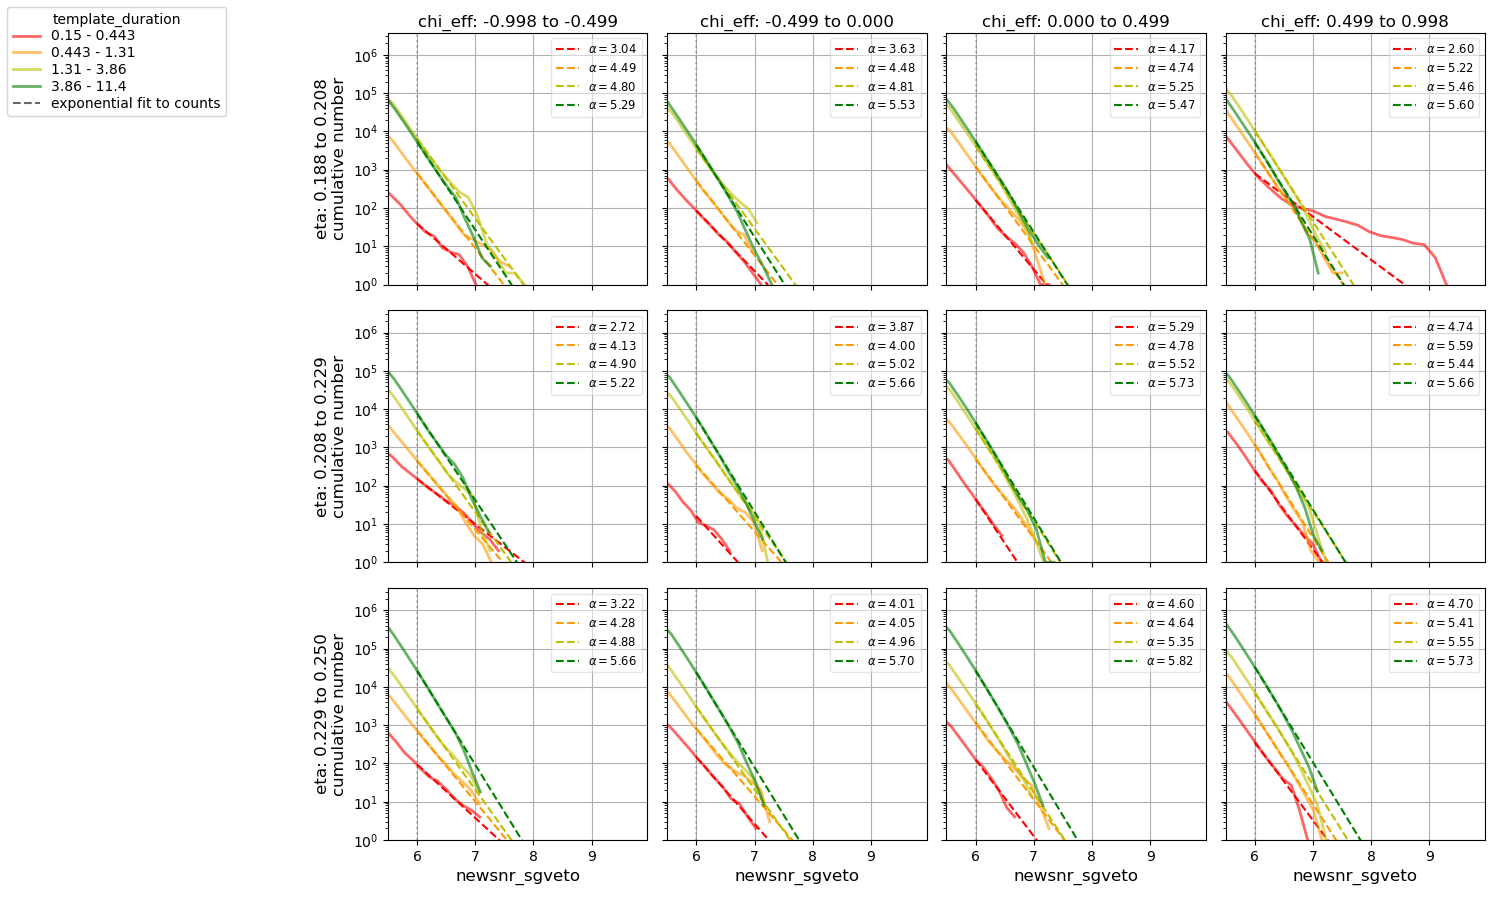
\includegraphics[width=1.0\linewidth]{images/5_pycbclive/L1-template_fits.png}
%     \label{fig:pycbclive-L1-fits}

%   \end{minipage}
%   \caption{The noise distributions for 12 discrete bins in the $\chi_{eff}$ and $\eta$ parameter space, with cumulative number on the vertical axis and $\rho_{new}$ on the horizontal axis. Each bin then has four discrete template duration bins plotted on top, alongside the exponential fit factor for each template bin. The top plot represents the triggers from the H1 detector and the bottom plot the L1 detector triggers.}
%   \label{fig:pycbclive-template-fits}
% \end{figure}
% %
% An example of template fits generated from a weeks worth of triggers can be seen in figure~\ref{fig:pycbclive-template-fits}. These are created from the first week of our injections testing data that was used to calculate increases in the search sensitivity from including the new ranking statistic components. From this figure we can see clearly the difference between `good' and `bad' template fits, a good fit is one with a steep slope (high $\alpha$) and the trigger distribution following closely to the slope line, bad fits have a shallow slop and poor fit to the line. It can be seen in figure~\ref{fig:pycbclive-template-fits} that we have binned over three parameters: $\chi_{eff}$, $\eta$, \verb|duration|, and we can see that high $\chi_{eff}$, low $\eta$ and short duration templates have the worst fits, meaning they are more likely to trigger on noise with a high SNR.

\section{\label{sec:pycbclive-injection-tests}Measuring Improvements in Search Sensitivity}

% Motivation for investigating the sensitivity increase
% How do we quantify sensitivity
To quantifiably demonstrate that the new additions to the ranking statistic have improved the live search we can investigate the differences in sensitivity when the PSD variation and noise falloff model are included. We quantify the sensitivity of the search by calculating the sensitive volume in which we can observe gravitational wave signals. The sensitive volume is calculated by measuring the detection efficiency of different distance bins that are taken from an injection set and then multiplying by the volume enclosed by the distance bins. The volume of each bin is then summed to find the total sensitive volume of the search~\cite{rw_snr_eq:2012}.

We can search through a period of data which contains an injections set with two instances of the PyCBC Live search, one containing the new ranking statistic additions and one representing the previous ranking statistic. The ratio of the new statistic sensitive volume to the previous statistic sensitive volume will indicate the change in sensitivity from including the new ranking statistic components.

% What is the injection set
We have chosen to test the ranking statistic changes to PyCBC Live using a smaller template bank than the PyCBC Live's current template bank, which contains over $730,000$ templates~\cite{PyCBC_Live:2018}. The focussed binary black hole search performed in the third observing run~\cite{PyCBC_focussed_bbh:2024} used a template bank with only $15,436$ templates with the drawback that we are only considering binary black hole signals. This smaller template bank uses fewer computational resources and allows a full week of data to be searched through with PyCBC Live in as little as $1$ day as the complete data is available to be processed as fast as possible. The focussed binary black hole search from the third observing run has an accompanying injection set with parameter value ranges~\cite{gwtc3:2023}:
%
% Table of injection parameter values
%
%
% Figure of the injections over the top of the template bank? To show good coverage
%
% DESCRIBE WHY THE TEST IS STILL REPRESENTATIVE JUST USING THE BBH INJECTIONS

% How did we test the search changes
As previously mentioned, the template fits are measured from the triggers found in the previous week to the week currently being searched through. Therefore to perform our injection set test we need to do an initial search with PyCBC Live using the original ranking statistic to generate a weeks worth of triggers and create template fit statistics from. The second week of data is then created containing a large number of gravitational wave injected signals that is searched through with PyCBC Live using both the original ranking statistic and the new ranking statistic. The two weeks of O3b gravitational wave data used lasted from 06 January 2020 23:59:42 to 20 January 2020 23:59:42 and, according to the gravitational wave catalogue for the third observing run, there were no real gravitational wave signals present. When the searches have completed analysing the second week of data we can directly count the number of injections found by both searches at different false-alarm rates at various intervals, if more injections are found with lower false-alarm rates then we have seen an overall improvement in the sensitivity of the search.

\section{\label{sec:pycbclive-sensitivity-improvements}Improvements in Sensitivity}

% What is significance, sensitivity and IFAR, why have we chosen the IFAR threshold we have chosen:
%  Ask Ian about the 2 detector vs 3 detector thing?
By adding the PSD variation and the noise falloff model to the ranking statistic we expect to see gravitational wave injections with a greater significance than before. This significance is determined by the false-alarm rate (FAR) of the injection, which has a direct mapping to the ranking statistic value, an event found with a FAR of $1$ per year would indicate that an event with the exact same parameters is expected to be seen in the data caused by non-astrophysical noise---not a real event. We commonly use the inverse false-alarm rate (IFAR) with units of $years$ and a large IFAR indicates a more confident detection. An IFAR threshold is chosen to separate events which are real from those that are false alarms, a balance must be made to avoid contaminating the detection catalogue with a large number of potential false alarms while not missing any real events. In this analysis we are considering only two detectors, allowing a great number of false-alarms from coincident noise when compared to a three detector configuration and therefore we have chosen a more conservative IFAR threshold of $1$ year. The current threshold for LIGO/Virgo alert generation is $1$ per $2$ months~\cite{PyCBC_Live:2018} from which gravitational wave searches will produce more potential gravitational wave events but these have additional stages with data quality checks from detector characterisation~\cite{O2O3_DetChar:2021} and parameter estimation~\cite{gwtc3:2023} which can also rule out false-alarms and prevent them from contaminating the catalogue.

% This is a low latency search so a threshold is hard to determine concretely.

% How do we compare sensitivity of the two searches using the significance of the injections
To measure the sensitivity improvement of the new ranking statistic we can directly compare the significance of each injection in both searches. The injection set is pre-weighted to ensure each injection represents the same volume, therefore instead of doing the distance binning described in section~\ref{sec:pycbclive-injection-tests} we can simply count the number of injections seen by each search in discrete IFAR bins and calculate the ratio of new search to original search.
% Sensitivity Increase Plot
%
% REPLACE WITH THE PSD VAR + TEMPLATE FITS + 0S VT RATIO
\begin{figure}
  \centering
  \begin{minipage}[t]{1.0\linewidth}
  
    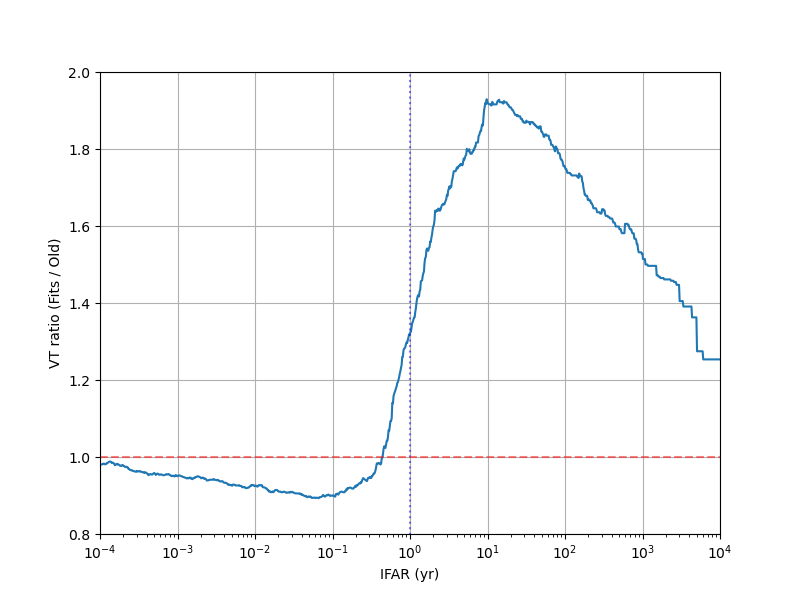
\includegraphics[width=1.0\textwidth]{images/5_pycbclive/ratio.png}
    \caption{The sensitive volume ratio between the new search and the old search. Calculated by sampling the number of injections found in both searches with an IFAR above the x value and dividing the number in the new search by the number from the old search.}
    \label{fig:pycbclive-psdvar-4s-sensitivity}

  \end{minipage}
\end{figure}
%
% Comments about the weird shape of the plot
Figure~\ref{fig:pycbclive-psdvar-4s-sensitivity} shows the sensitivity ratio plot comparing the new statistic search to the original statistic search. We see $35\%$ more injections with an IFAR greater than our threshold of $1$ year which is a very large increase in sensitivity however we have two strange features to to the sensitivity plot, the large decrease in sensitivity at the IFAR $= 0.1$ year mark and the extremely large increase at the IFAR $= 10$ year point. To understand the shape of the sensitivity curve we can look at how the new additions to the ranking statistic are changing the significance on an injection by injection basis.

\section{\label{sec:pycbclive-injection-investigations}Changes in Injection Significance}

% How do IFAR and Significance relate
The ranking statistic assigned to each event can be mapped directly to IFAR, shown in figure~ADD. Changing the ranking statistic calculation will lead to incomparable values between searches but the IFAR values can still be compared. The PyCBC Live search will matched filter the template bank and the data and where the resulting SNR and new SNR is above pre-defined thresholds (both $4.5$ in the fourth observing run) the trigger is kept. The coincidence ranking statistic value is calculated and then an IFAR is assigned to the event. The initial SNR values are the same between the two searches because these depend only on template and data but the new SNR value depends on the single detector ranking statistic which has the addition of PSD variation in our new statistic, therefore it is possible for the PSD variation to prevent the saving of a trigger due to the new SNR being re-weighted below the threshold.
%
% Plot of ranking statistic and IFAR mapping like in figure 2 https://ar5iv.labs.arxiv.org/html/1805.11174
%

% How does the new statistic change the injections found
We can plot the IFAR value of each injection that has been found in both searches, seen in 
% REPLACE WITH THE PSD VAR + TEMPLATE FITS + 0S VT IFAR VS IFAR
figure~\ref{fig:pycbclive-ifar-ifar-psdvar-4s}.
%
\begin{figure}
  \centering
  \begin{minipage}[t]{1.0\linewidth}
  
    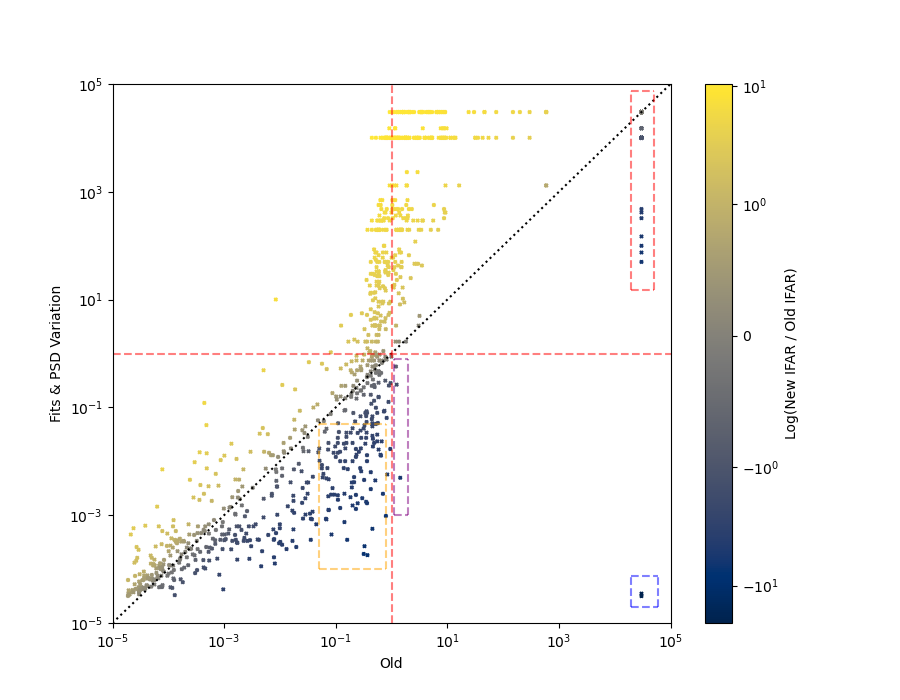
\includegraphics[width=1.0\textwidth]{images/5_pycbclive/psdvar_4s_ifar_vs_ifar_regions.png}
    \caption{Each point represents an injection in the injection set. The y values are the IFAR recorded from the search including the new noise falloff model and PSD variation in the ranking statistic, and the x value is the IFAR value when found with the original statistic. The colour bar represents the log difference in the IFAR of the two searches. The dashed line at $y=x$ represents an injection having the same IFAR in both the new and the old search. The vertical and horizontal lines represent an IFAR threshold of $1$ year, above which an injection might be considered real.}
    \label{fig:pycbclive-ifar-ifar-psdvar-4s}

  \end{minipage}
\end{figure}
%
Within figure~\ref{fig:pycbclive-ifar-ifar-psdvar-4s} we have plotted a vertical and horizontal dotted line at an IFAR of $1$ year and we can be split into four quadrants: top-left, injections originally found below the IFAR threshold with the old statistic and now found above it with the new statistic; top-right, injections found in both searches; bottom-left, injections below the threshold in both searches; bottom-right, injections originally found above the IFAR threshold but now found below threshold with the new statistic. Another line has been plotted at y=x, injections above this line ($y > x$) have been found with a larger IFAR with the new statistics and injections below ($y < x$) have been found with a lower IFAR with the new statistic.

Figure~\ref{fig:pycbclive-psdvar-4s-sensitivity} highlighted two IFAR values of $0.1$ and $10$ years. We can look at figure~\ref{fig:pycbclive-ifar-ifar-psdvar-4s} and identify the regions responsible for the shape of the sensitivity curve. There are a greater number of injections found below the $y = x$ line at an IFAR of $0.1$ years and the new statistic has a much greater number of injections above the $10$ year mark when compared to the original statistic.

To further understand the shape of the sensitivity curve we can do a region-by-region investigation into some of the downranked regions shown in the IFAR vs IFAR figure. We have highlighted four dashed boxes which contains some downranked injections of interest and we need to understand why these regions have been down-ranked when using the new statistic and if there are any changes that can be made to the ranking statistic to avoid the downranking.

\section{\label{pycbclive-ignoring-psdvar}Does PSD Variation Improve Sensitivity}

The injections shown in figure~\ref{fig:pycbclive-ifar-ifar-psdvar-4s} that lie below the $y = x$ diagonal line have been found with a lower significance when including the PSD variation and the noise falloff model in the ranking statistic. We can separate the new additions and investigate the individual contributions to the increase sensitivity.

The PSD variation measures the non-stationary noise in the data and applies a weighting to the new SNR value calculated by the single detector ranking statistic. We have previously described how the PyCBC Live search re-calculates the PSD every stride and replaces the current used PSD when the BNS distance of the new PSD differs from the current PSD's by more than $1\%$.

We can produce the figure~\ref{fig:pycbclive-ifar-ifar-psdvar-4s} but compare the IFAR of the found injections when the search includes both the noise falloff model and the PSD variation versus the search which includes only the noise falloff model, this will reveal how the PSD variation is effecting the significance of the injections. This comparison is shown in figure~\ref{fig:pycbclive-ifar-ifar-fits-psdvar}.
% REPLACE WITH THE PSD VAR + TEMPLATE FITS + 0S IFAR VS IFAR VS TEMPLATE FITS
%
\begin{figure}
       \centering
    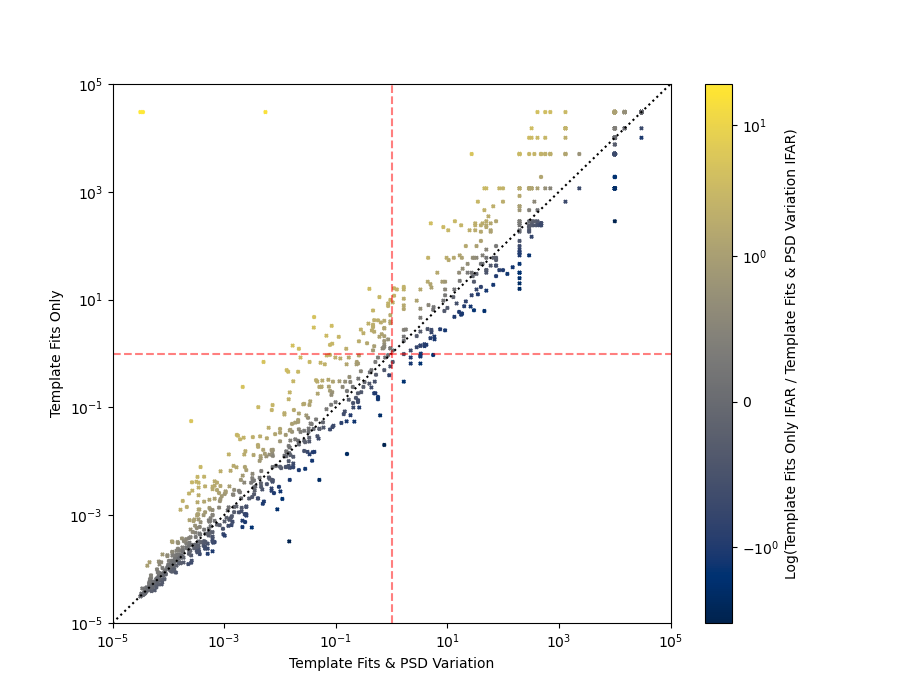
\includegraphics[width=1\textwidth]{images/5_pycbclive/fits_psdvar_comparison_ifar_vs_ifar_diff.png}
    \caption{}
    \label{fig:pycbclive-ifar-ifar-fits-psdvar}
\end{figure}
%
In this comparison, $550$ injections were found with a higher significance when \textbf{not} including PSD variation, $399$ were found with a higher IFAR when including PSD variation and $326$ were found with the same IFAR. We can see from figure~\ref{fig:pycbclive-ifar-ifar-fits-psdvar} that there is a greater dispersion of injections found above the line when compared to those found below it, meaning when an injection is found above the diagonal line it is found with a greater significance difference than when it is found below the line. Alongside this general trend we can see a few injections in the top-left of the plot which have had a very large increase in significance when we do not include PSD variation in the statistic. These injections in the top left correspond to the blue box in the bottom-right of figure~\ref{fig:pycbclive-ifar-ifar-psdvar-4s}.

We can plot the IFAR vs IFAR plot for the search including only the noise falloff model in the ranking statistic compared to the original search, seen in figure~\ref{fig:pycbclive-ifar-ifar-fits-only-4s}, which can be directly compared to figure~\ref{fig:pycbclive-ifar-ifar-psdvar-4s}. As well as this we can plot the sensitivity ratio of the search including both new ranking statistic components and the search including only the noise falloff model, shown in figure~\ref{fig:pycbclive-vt-ratio-f-fo}.
%
% REPLACE WITH THE PSD VAR + TEMPLATE FITS + 0S VS TEMPLATE FITS VT RATIO
\begin{figure}
       \centering
    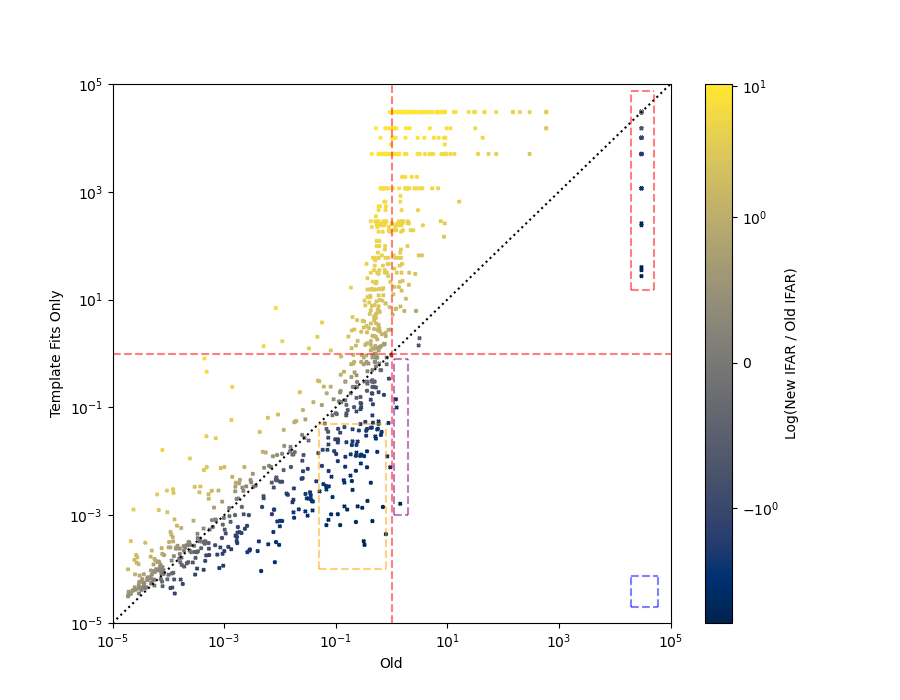
\includegraphics[width=1.0\textwidth]{images/5_pycbclive/fits_only_4s_ifar_vs_ifar_regions.png}
    \caption{}
    \label{fig:pycbclive-ifar-ifar-fits-only-4s}
\end{figure}
%
\begin{figure}
       \centering
    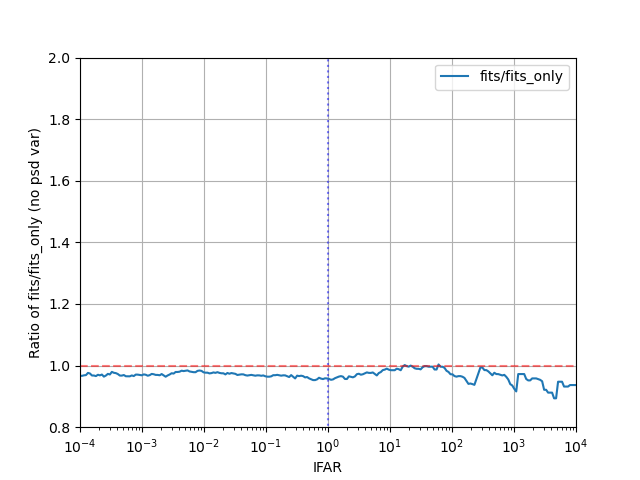
\includegraphics[width=1.0\textwidth]{images/5_pycbclive/f_vs_fo.png}
    \caption{}
    \label{fig:pycbclive-vt-ratio-f-fo}
\end{figure}
%
From these comparisons and the clear decrease in sensitivity when using the PSD variation in the ranking statistic in the PyCBC Live search we make the choice to not use the PSD variation in the ranking statistic going forward.

\section{\label{pycbclive-investigating-regions}Investigating Downranked Regions}

We have investigated the effect of including the PSD variation in the ranking statistic and concluded that it will not enter the ranking statistic going forward. However, when looking at the sensitivity ratio for the ranking statistic including only the noise falloff model against the original statistic (figure~ADD) we can see that the $0.1$ and $10$ year IFAR bumps are still present.
%
% FIGURE FOR THE VT RATIO MENTIONED ABOVE
%
Looking at figure~ADD there are still three regions to investigate and explain the cause of the downranking. The yellow region is of particular interest as being the one responsible for the $0.1$ year dip in the sensitivity ratio figure.


%%%%%%%%%%%%%%%%%%%%%%%%%%%%%%%%%%%%%%%%%%%%%%%%%%%%%%%%%%%%
\subsection{\label{sec:pycbclive-poor-temp-fits}Templates with High Noise Rates}

% Log(noise rate) equation
% Combined log(noise rate) equation
% Low Alpha + High Rate == High Combined Log(noise rate)
% Plot Alpha vs Rate, colour Log(noise rate)
% Plot Alpha vs SNR, colour Log(noise rate)

% What identifies a template as having a high noise rate
The new noise falloff model in the ranking statistic allows us to treat individual templates differently depending on historical trigger rates. This allows us to downrank poorly performing templates which will frequently trigger on non-gaussian noise with a high SNR. As describe in equation~ADD, the noise falloff model is characterised by an exponential fit to the slope of the trigger distribution and is quantified by the exponential fit factor, $\alpha$, and the rate of triggers above a threshold, $\mu$. Therefore, using these two parameters we must be able to differentiate between which templates do and which templates do not trigger frequently on noise.

All templates in the bank will trigger on noise in our data, from both Gaussian noise and glitches, and after applying all signal consistency tests these triggers might still might have new SNR of over $8$. Figure~\ref{pycbclive-template-fits} shows the trigger distributions for the template bank which has been split into $12$ discrete bins. The exponential fit factors of template duration bins are plotted on top of these.
%
\begin{figure}
  \centering
  \begin{minipage}[t]{1.0\linewidth}
  
    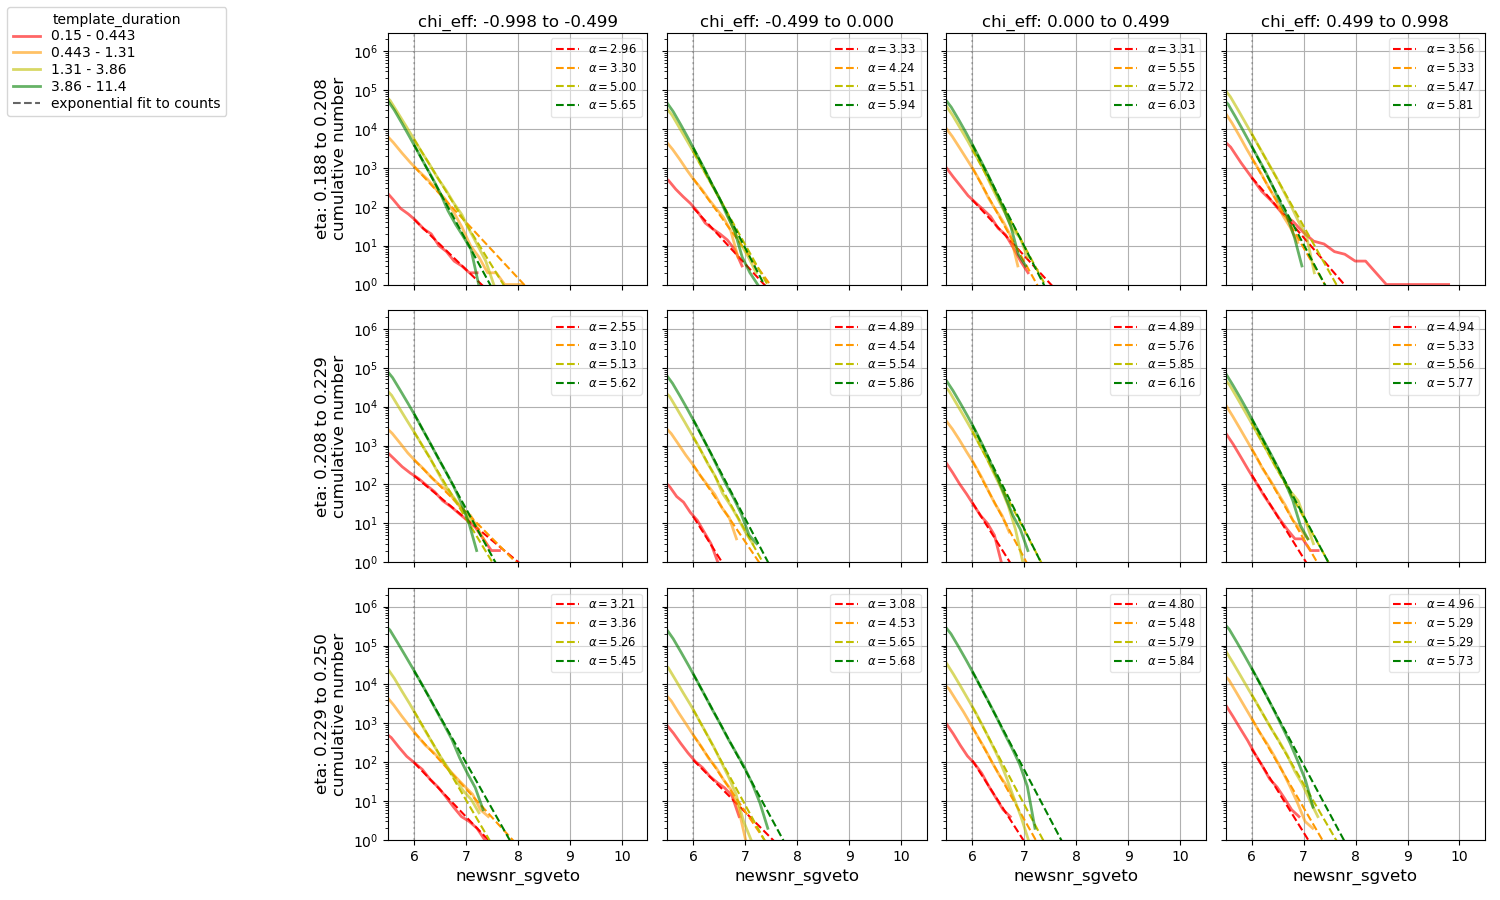
\includegraphics[width=1.0\textwidth]{images/5_pycbclive/H1-template_fits.png}
    \label{fig:pycbclive-H1-fits}

  \end{minipage}
  \caption{The noise distributions for 12 discrete bins in the $\chi_{eff}$ and $\eta$ parameter space, with cumulative number on the vertical axis and $\rho_{new}$ on the horizontal axis. Each bin then has four discrete template duration bins plotted on top, alongside the exponential fit factor for each template bin.}
  \label{fig:pycbclive-template-fits}
\end{figure}
%
This figure shows the difference in exponential fit slopes for the varying template bins and it can be seen that the bins which trigger more frequently with a higher new SNR have shallower slopes (lower $\alpha$) compared to the steeper slopes (higher $\alpha$) of some other bins. Equation~\ref{eqn:pycbclive-single-log-noise-rate} shows that higher $\alpha$ values correspond to a lower noise event rate density and lower $\alpha$ and higher $\mu$ values produce a higher noise event rate density.

When a template frequently triggers on noise and it is downranked in the ranking statistic but it is now possible that real gravitational wave signals belonging to template with poor fits will be downranked if they have lower $\rho_{new}$ values. To visualise how $\alpha$ and $\mu$ contribute to the noise event rate density (equation~\ref{eqn:pycbclive-single-log-noise-rate}) we plot the single detector log noise event rate density for $\alpha$ values $1.5$ to $6.0$ and $\mu$ values $5$ to $45$ which represent the range of values that we have seen in our test, this can be seen in figure~\ref{fig:pycbclive-log-noise-static-snr} where we have used a static $\rho_{new}$ of $10.0$. It can be seen that a higher $\alpha$ values have a greater effect on the log noise event rate density and while $\mu$ has some effect ($ + \log(\mu)$ in equation~\ref{eqn:pycbclive-single-log-noise-rate}) its contribution is minimal.
%
\begin{figure}
    \centering
    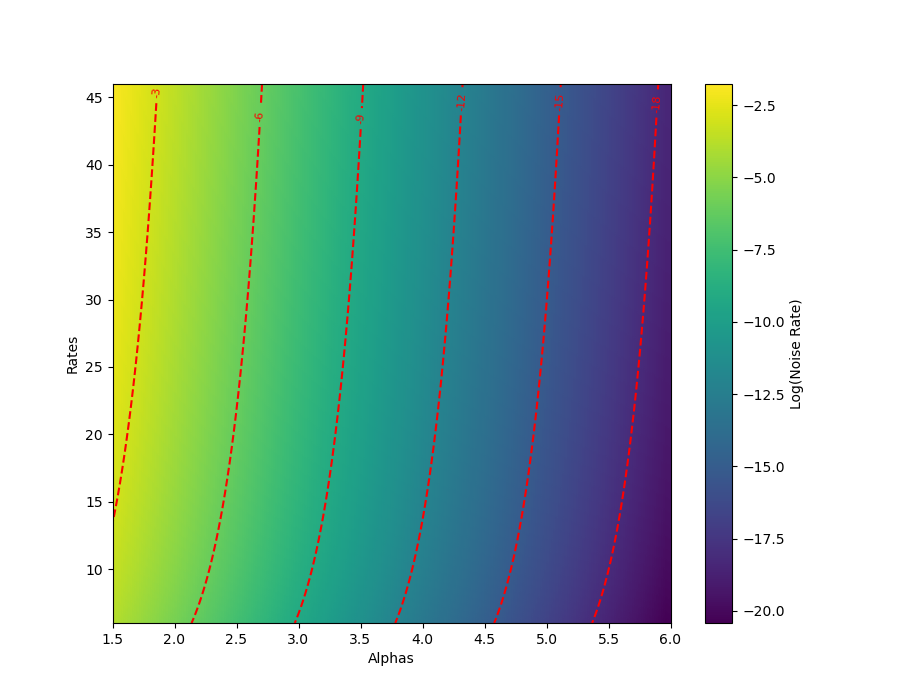
\includegraphics[width=1\textwidth]{images/5_pycbclive/lognoise_alpha_rate.png}
    \caption{}
    \label{fig:pycbclive-log-noise-static-snr}
\end{figure}
%
\begin{figure}
    \centering
    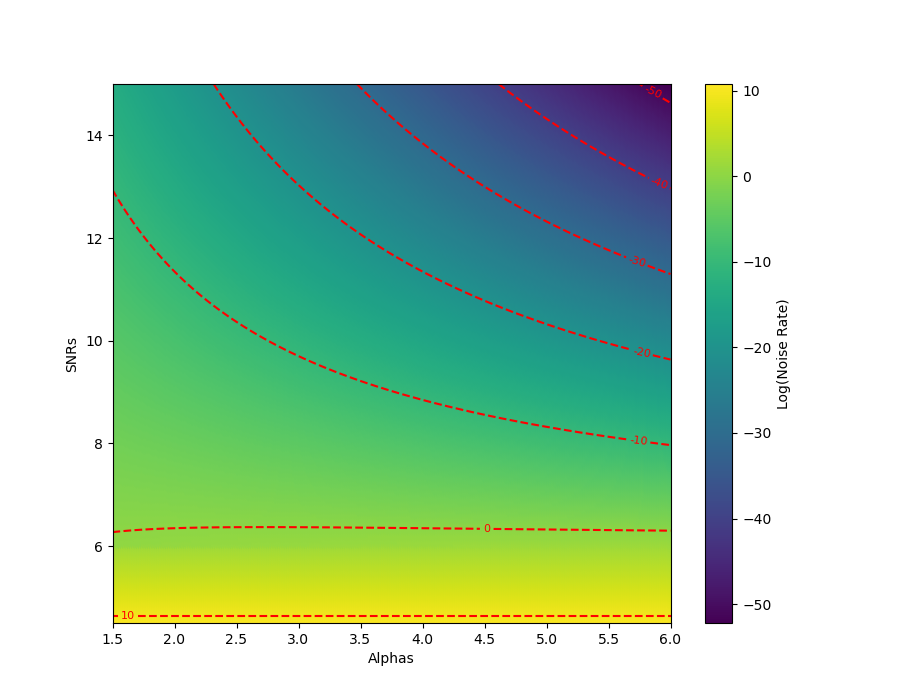
\includegraphics[width=1\textwidth]{images/5_pycbclive/lognoise_alpha_snr.png}
    \caption{}
    \label{fig:pycbclive-log-noise-static-rate}
\end{figure}
%
We produce the same figure but instead set $\mu$ to the benchmark log noise rate, $-14.6$, which is the log of a representative noise trigger rate and originates from the second observing run, figure~\ref{fig:pycbclive-log-noise-static-rate}. This figure shows us how SNR changes the log noise rate alongside $\alpha$, a black dashed line has been plotted at $\rho_{new} = 6.0$ due to triggers below this SNR threshold all being assigned $\alpha = 6.0$, therefore the log noise rate values below this threshold are the same for all values on $\alpha$ on our plot. We can clearly see a strong correlation between SNR and log noise rate with a heavy dependency on $\alpha$, to the point where high SNR triggers with low $\alpha$--while still significant--are a lot worse than those with high $\alpha$.

% Plot IFAR vs IFAR, colour alpha
% Plot IFAR vs IFAR, colour rate
% Plot IFAR vs IFAR, colour H1 log(noise rate)
% Plot IFAR vs IFAR, colour L1 log(noise rate)
% Plot IFAR vs IFAR, colour Combined log(noise rate)

We can plot the IFAR vs IFAR distribution for the injection set for a single detector's $\alpha$, $\mu$ and log noise rate to see if there is any clear dependence on the template fit parameters, seen in figures~\ref{fig:pycbclive-ifar-ifar-h1-alpha},~\ref{fig:pycbclive-ifar-ifar-h1-rate}, and~\ref{fig:pycbclive-ifar-ifar-h1-log-noise-rate}.
%
\begin{figure}
    \centering
    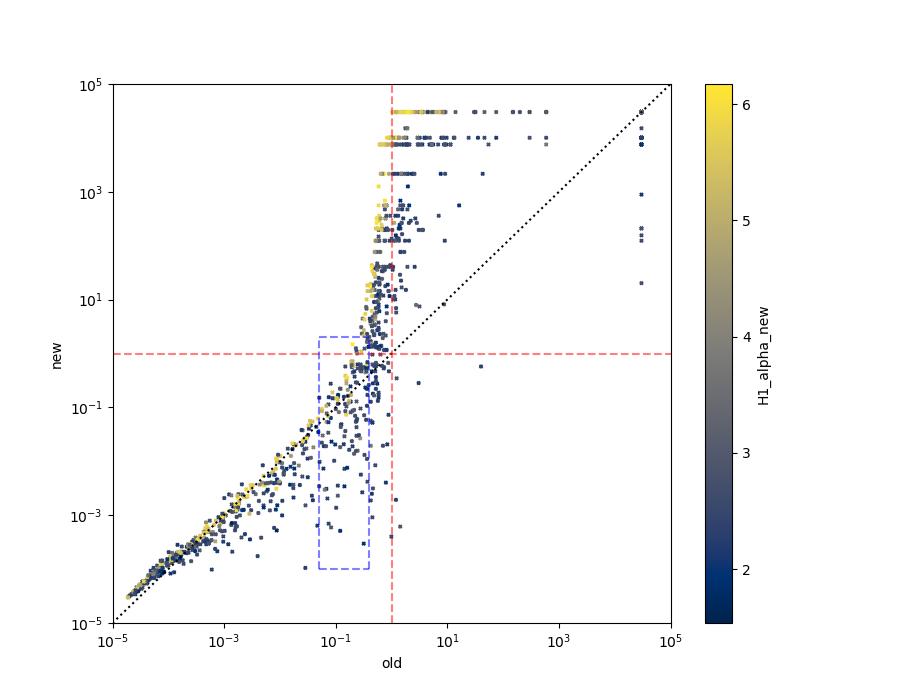
\includegraphics[width=\textwidth]{images/5_pycbclive/all_full_h1_alpha.png}
    \caption{}
    \label{fig:pycbclive-ifar-ifar-h1-alpha}
\end{figure}
%
\begin{figure}
    \centering
    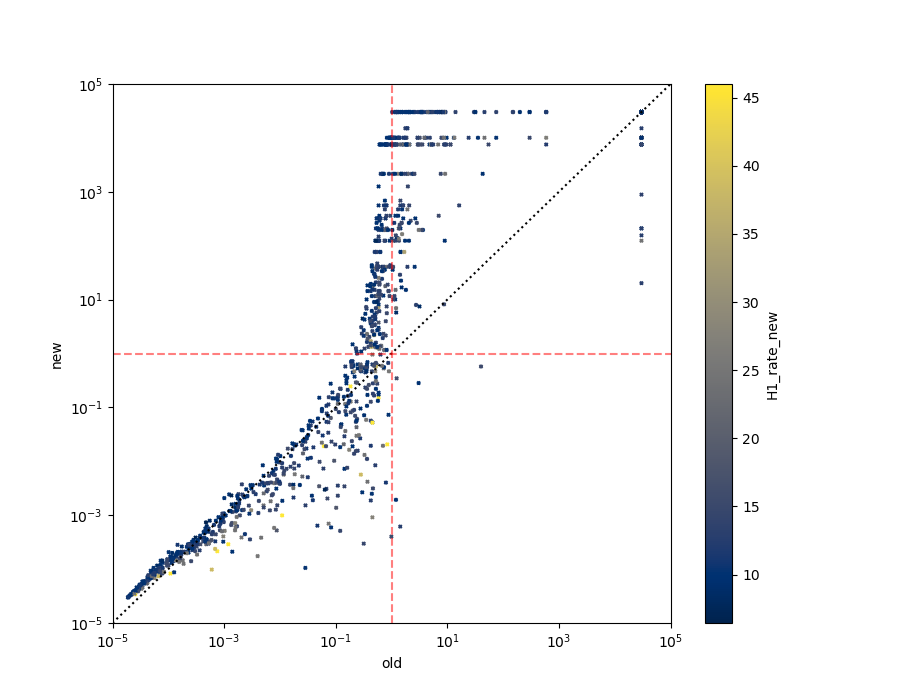
\includegraphics[width=\textwidth]{images/5_pycbclive/all_full_h1_rate.png}
    \caption{}
    \label{fig:pycbclive-ifar-ifar-h1-rate}
\end{figure}
%
\begin{figure}
    \centering
    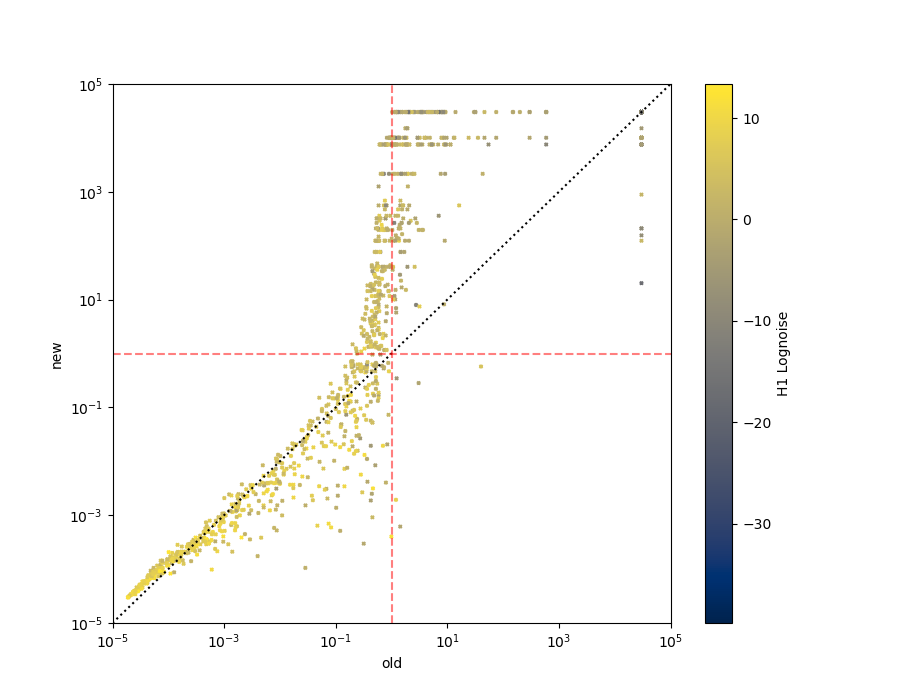
\includegraphics[width=\textwidth]{images/5_pycbclive/all_full_h1_lognoise.png}
    \caption{}
    \label{fig:pycbclive-ifar-ifar-h1-log-noise-rate}
\end{figure}
%
It is not clear from these figures that $\alpha$ and $\mu$ are having a large effect on the log noise shown in the bottom figure. There is a curve of high $\alpha$ points above the $y=x$ line in the top figure but we would hope to see a better distinction between higher and lower $\alpha$ values corresponding to improved and worsened IFAR values. As mentioned before and reinforced by the middle plot, the rate has a small effect on the log noise rate and low rate values are far more common than high ones, the high ones are located in the bottom left quadrant below the $y=x$ line.

To investigate this further we can look at the distribution of combined log noise rates, shown in figure~\ref{fig:pycbclive-ifar-ifar-comb-log-noise-rate}.
%
\begin{figure}
  \centering
  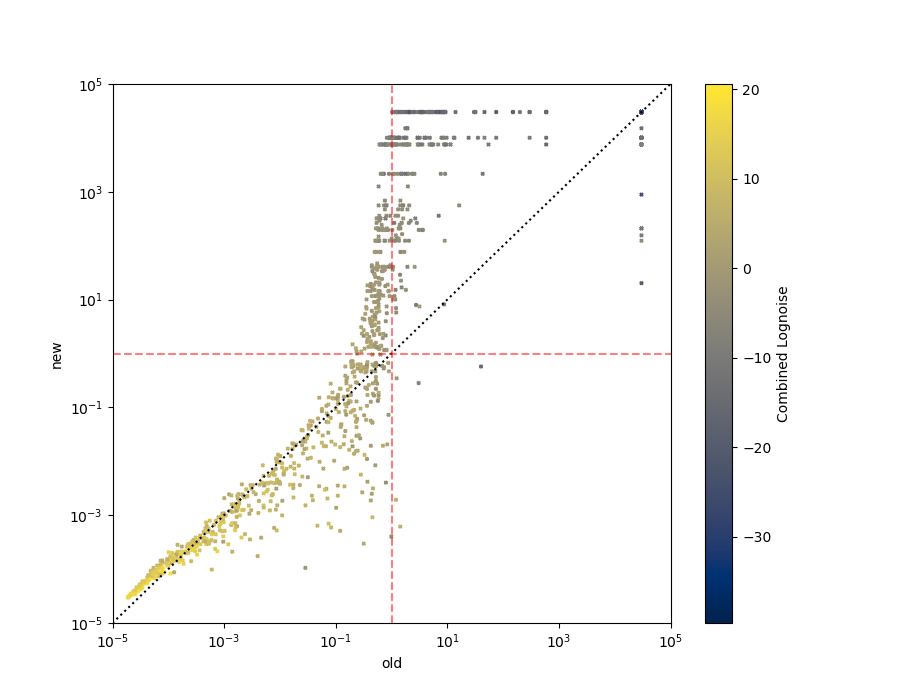
\includegraphics[width=1\textwidth]{images/5_pycbclive/all_full_comb_lognoise.png}
  \caption{}
  \label{fig:pycbclive-ifar-ifar-comb-log-noise-rate}
\end{figure}
%
From this figure we can see a much clearer distinction between higher and lower noise rates and how this is affecting the ranking statistic, where we expect a lower noise rate to improve the ranking statistic. However, looking at this plot we can see that combined log noise rate isn't the entire explanation for improved significance, we can see clearly there are some low noise rate injections below the $y=x$ line which should have caused an increase in the significance but we have seen a drop. Therefore we must investigate other components of the ranking statistic and how these build up our ranking statistic model.

\subsection{\label{sec:pycbclive-diff-triggers}Different Triggers Selected by Each Search}

% Different triggers == different templates
% Different templates == different signal rate
% Plots of same trigger
% Plots of different trigger
% Plots of Total Ranking Statistic distribution

The inclusion of the template fits will quantitatively change how the combined noise rate contributes to the ranking statistic but, there is another component to the ranking statistic that can change. Our ranking statistic is a simple sum of four separate components, the two that can change are the combined log noise rate and the log signal rate, therefore we can reduce the new statistic ranking statistic equation simply to $R = log(r_s) - log(r_n)$.

Therefore we can look at the scenario where the log signal rate has also changed between searches. The log signal rate is dependent on four parameters of a trigger: $\rho$ (note, not $\rho_{new}$), $\phi$, $t_{c}$ and, $\verb|sigmasq|$. We expect the phase, $\phi$, and time, $t_{c}$, differences between detectors to be determined by the detector's location and the source's sky location and orientation. Therefore, for a particular trigger we expect this to be the same in both searches and the log signal rate would be the same for the same trigger.

If we see a different trigger between searches this opens up potential for a difference in the log signal rate to effect the ranking statistic. However, this also poses the question of why the search has chosen a different trigger between searches? The event with the highest ranking statistic is chosen as the best event for a particular injection and therefore we come back to the specific components of the ranking statistic changing between searches but also the formulation of the ranking statistic itself. 

% Changes in ranking statistic, balance between logr_s and logr_n
% Plot signal rate for same trigger, IFAR vs IFAR
% Plot signal rate for different trigger, IFAR vs IFAR
% Plot new ranking statistic total, IFAR vs IFAR
% Plot old ranking statistic total, IFAR vs IFAR

We can directly compare the equation for the old ranking statistic,
%
\begin{equation}
    R_{old} = \sqrt{2(ln(r_n) + ln(r_s))}
\label{eqn:pycbclive-old-ranking-statistic}
\end{equation}
%
to that of the new ranking statistic,
%
\begin{equation}
    R_{new} =  ln(r_s) - ln(r_n)
\label{eqn:pycbclive-new-ranking-statistic-simple}
\end{equation}
%
and we can immediately see a clear difference in how both the noise rates and signal rates contribute to the ranking statistic value. It is due to these formulations that we cannot directly compare ranking statistic values between searches to identify why the significance of injections has changed.

Different triggers in the new statistic search have therefore been found with a higher ranking statistic when compared to the trigger found by the original search, an example of one of these is seen in table~\ref{tab:pycbclive-200-new-stat},
%TABLE
%
\begin{table}[ht]
    \centering
    \setlength{\tabcolsep}{3pt}
    \begin{minipage}{0.48\textwidth}
        \centering
        \rowcolors{2}{white}{lightgray}
        \begin{adjustbox}{minipage=\linewidth-0cm, margin=-5.5cm 0pt 0pt 0cm}
        \begin{tabular}{lcc}
            \toprule
            \textbf{Inj Idx = 200} & \textbf{Old Trigger} & \textbf{New Trigger} \\
            \midrule
            Comb Log(Noise Rate)  & -15.53 & -18.79 \\
            Log(Signal Rate) & -15.77 & -15.67 \\
            $R_{new}$ & -0.24 & 3.12 \\
            \bottomrule
        \end{tabular}
        \end{adjustbox}
        \caption{}
        \label{tab:pycbclive-200-new-stat}
    \end{minipage}
    \hfill
    \begin{minipage}{0.48\textwidth}
        \centering
        \rowcolors{2}{white}{lightgray}
        \begin{tabular}{lcc}
            \toprule
            \textbf{Inj Idx = 445} & \textbf{Old Trigger} & \textbf{New Trigger} \\
            \midrule
            Comb Log(Noise Rate)  & -12.96 & -12.69 \\
            Log(Signal Rate) & -4.40 & -2.74 \\
            $R_{new}$ & 8.56 & 9.95 \\
            \bottomrule
        \end{tabular}
        \caption{}
        \label{tab:pycbclive-445-new-stat}
    \end{minipage}
\end{table}
%
It can be seen that the signal rate contribution is marginally improved in the new trigger but the noise rate contribution is the majority of the increase in the ranking statistic. Table~\ref{tab:pycbclive-445-new-stat} shows a different case where the noise rates of the old and new trigger are similar but by selecting a different template we have found an improved signal rate causing the increase in the ranking statistic. We can also show the ranking statistic values found by the old statistic to see why these triggers are different, tables~\ref{tab:pycbclive-200-old-stat} and~\ref{tab:pycbclive-445-old-stat} show these.
%TABLE
%
\begin{table}[ht]
    \centering
    \setlength{\tabcolsep}{5pt}
    \begin{minipage}{0.48\textwidth}
        \centering
        \rowcolors{2}{white}{lightgray}
        \begin{adjustbox}{minipage=\linewidth-0cm, margin=-5cm 0pt 0pt 0cm}
        \begin{tabular}{lcc}
            \toprule
            \textbf{Inj Idx = 200} & \textbf{Old Trigger} & \textbf{New Trigger} \\
            \midrule
            $\rho_{new, H1}$  & 15.06 & 13.50 \\
            $\rho_{new, L1}$   & 6.67 & 6.58 \\
            $\rho_{new, H1}^2 + \rho_{new, L1}^2$   & 271.29 & 225.25 \\
            Log(Signal Rate) & -15.77 & -15.67 \\
            $R_{new}$ & 15.48 & 13.93 \\
            \bottomrule
        \end{tabular}
        \end{adjustbox}
        \caption{}
        \label{tab:pycbclive-200-old-stat}
    \end{minipage}%
    \hfill
    \begin{minipage}{0.48\textwidth}
        \centering
        \rowcolors{2}{white}{lightgray}
        \begin{tabular}{lcc}
            \toprule
            \textbf{Inj Idx = 445} & \textbf{Old Trigger} & \textbf{New Trigger} \\
            \midrule
            $\rho_{H1,new}$  & 10.44 & 10.78 \\
            $\rho_{L1,new}$   & 8.14 & 7.16 \\
            $\rho_{H1,new}^2 + \rho_{L1,new}^2$   & 175.25 & 167.47 \\
            Log(Signal Rate) & -4.40 & -2.74 \\
            $R_{new}$ & 12.90 & 12.73 \\
            \bottomrule
        \end{tabular}
        \caption{}
        \label{tab:pycbclive-445-old-stat}
    \end{minipage}
\end{table}
%
We can plot the IFAR vs IFAR distribution with the combined log signal rate as the colour of each injection but we can further split this into two groups, those found with the same trigger in both searches (figure~\ref{fig:pycbclive-ifar-ifar-same-trigs-comb-log-noise-rate}) and those found with different triggers figure~\ref{fig:pycbclive-ifar-ifar-diff-trigs-comb-log-noise-rate}. These plots show there is no clear difference in the combined log noise values associated with injections found with the same or different triggers between searches.
% PLOT
% SAME TRIGGER, LOG SIG RATE
% DIFF TRIGGER, LOG SIG RATE
%
\begin{figure}
    \centering
    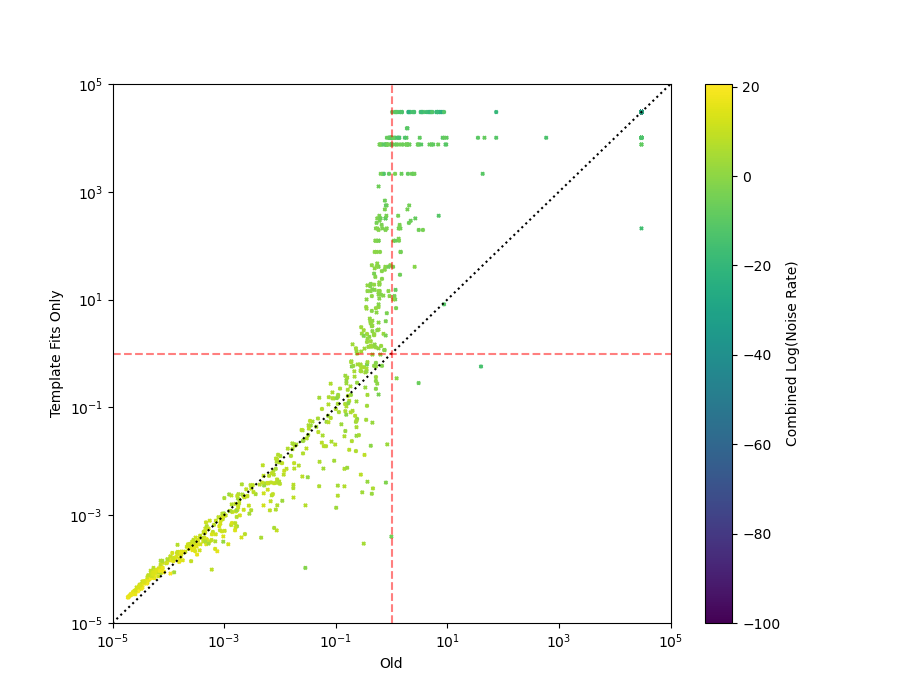
\includegraphics[width=1\textwidth]{images/5_pycbclive/ifar_vs_ifar_same_template_ids_comb_log_noise.png}
    \caption{}
    \label{fig:pycbclive-ifar-ifar-same-trigs-comb-log-noise-rate}
\end{figure}
%
\begin{figure}
    \centering
    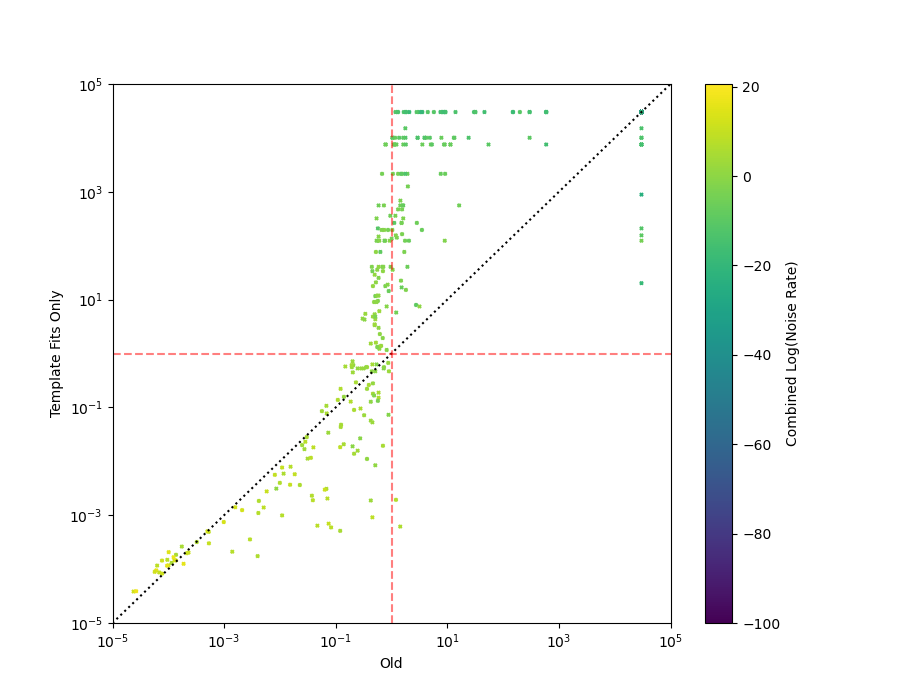
\includegraphics[width=1\textwidth]{images/5_pycbclive/ifar_vs_ifar_diff_template_ids_comb_log_noise.png}
    \caption{}
    \label{fig:pycbclive-ifar-ifar-diff-trigs-comb-log-noise-rate}
\end{figure}
%
Another plot we can look into is how these injections are distributed in both the old and new ranking statistic values. Figures~\ref{fig:pycbclive-ifar-ifar-old-stat} and~\ref{fig:pycbclive-ifar-ifar-new-stat} show the IFAR vs IFAR plot with the top plot showing the injections coloured with their old statistic value and the bottom plot showing them coloured with their new statistic value. The progression of the colours can be seen as corresponding to the $x$ and $y$ directions as plotted, this is because there is a direct mapping between ranking statistic and IFAR for each search. In both figures, ranking statistic values above the colourbar max were set equal to the max to prevent large ranges of statistic values drowning out the smaller differences.
% PLOT
% OLD STAT
% NEW STAT
%
\begin{figure}
    \centering
    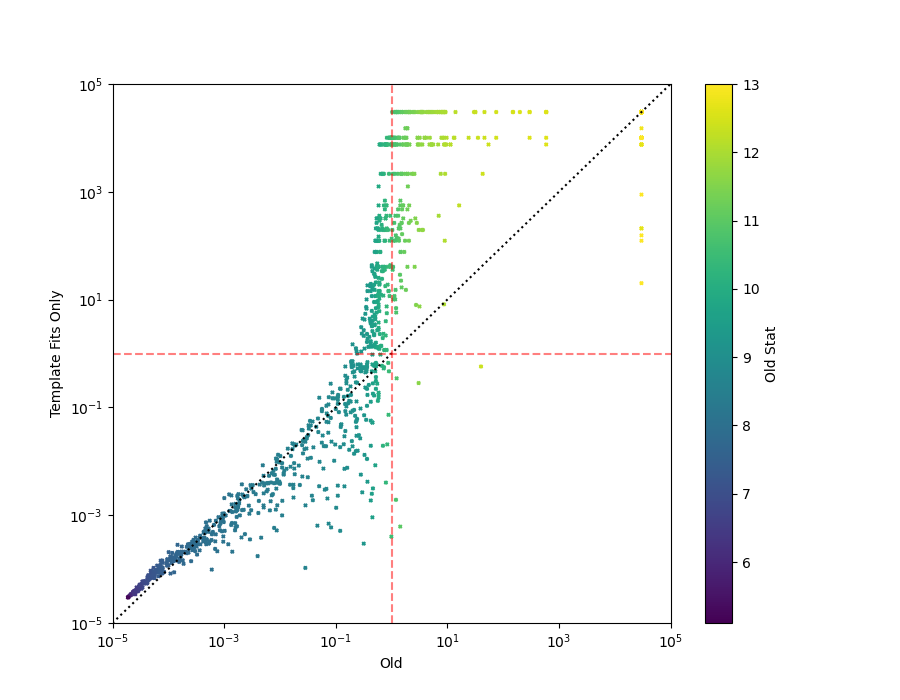
\includegraphics[width=1\textwidth]{images/5_pycbclive/ifar_vs_ifar_old_stat.png}
    \caption{}
    \label{fig:pycbclive-ifar-ifar-old-stat}
\end{figure}
%
\begin{figure}
    \centering
    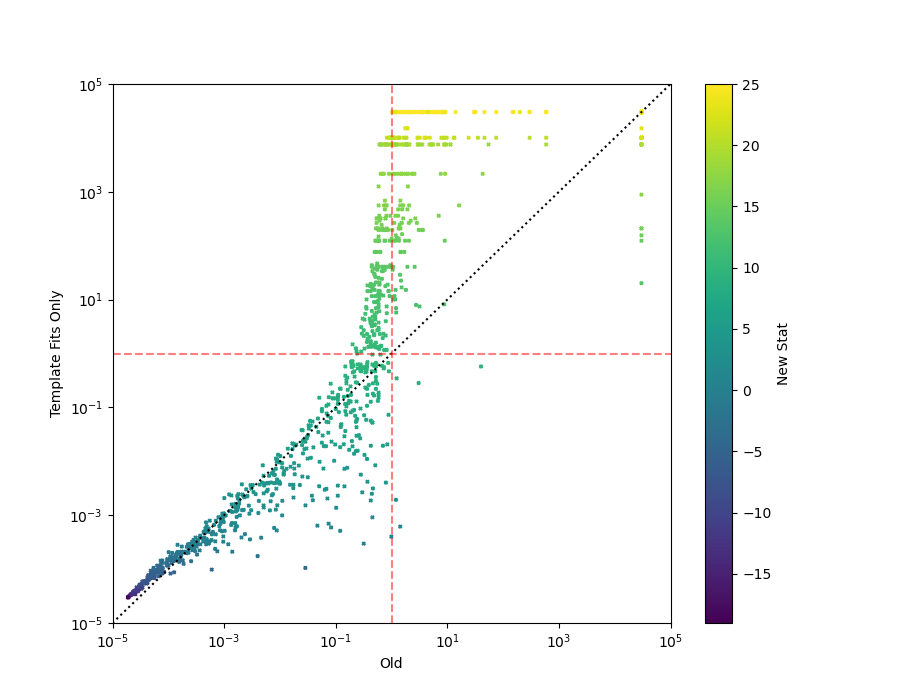
\includegraphics[width=1\textwidth]{images/5_pycbclive/ifar_vs_ifar_new_stat.png}
    \caption{}
    \label{fig:pycbclive-ifar-ifar-new-stat}
\end{figure}
%

\subsection{\label{sec:pycbclive-noise-contrib}Differences in the Noise Rate Contribution}

% Old Statistic Noise Rate

The old statistic assumes Gaussian, stationary noise for the noise rate. Therefore, we can model the noise rate for each detector as a Gaussian distribution,
%
\begin{equation}
    r_{n,det} \propto \exp \left( -\frac{(\rho_d - \mu)^2}{2 \sigma^2} \right)
    \label{eqn:pycbclive-old-noise-rate}
\end{equation}
%
and the combined noise rate is the product of both detector noise rates,
%
\begin{equation}
    r_{n,comb} \propto \exp \left( -\frac{(\rho_{H}^{2} + \rho_{L}^{2})}{2} \right) ,
    \label{eqn:pycbclive-old-comb-noise-rate}
\end{equation}
%
when the mean is equal to 0 and the variance 1. It can be seen from equation~\ref{eqn:pycbclive-old-comb-noise-rate} that the the rate of noise events decreases exponentially with the sum of the SNR$^{2}$s of the triggers.

% New Statistic Noise Rate
The new statistic attempts to model the distribution of the noise events using template fits and therefore the noise is not assumed to be Gaussian or stationary. We can plot the combined log noise rate (equation~\ref{eqn:pycbclive-comb-log-noise-rate}) as a function of detector SNR with the old statistic combined log noise rate shown in figure~\ref{fig:pycbclive-comb-lognoise-old} and the new statistic in figure~\ref{fig:pycbclive-comb-lognoise-new}.
%
\begin{figure}
    \centering
    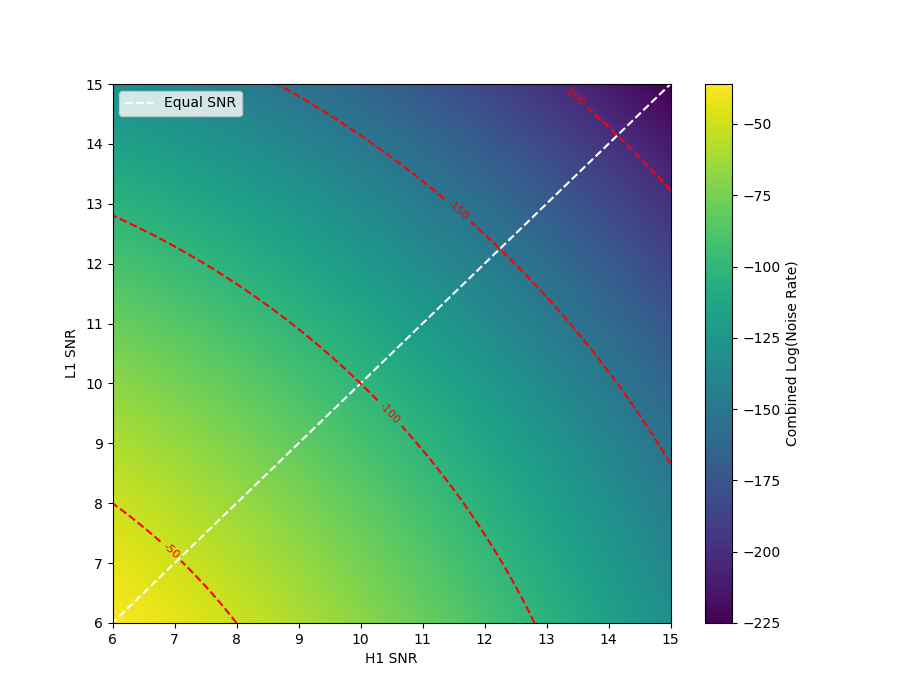
\includegraphics[width=1\textwidth]{images/5_pycbclive/comb_lognoise_old_stat.png}
    \caption{}
    \label{fig:pycbclive-comb-lognoise-old}
\end{figure}
%
\begin{figure}
    \centering
    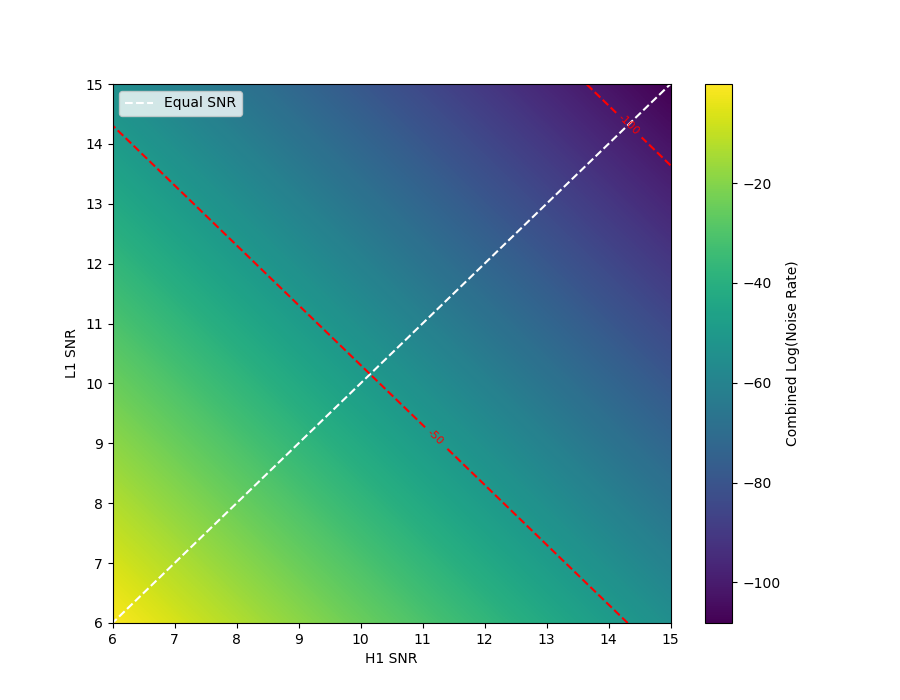
\includegraphics[width=1\textwidth]{images/5_pycbclive/comb_lognoise_new_stat.png}
    \caption{}
    \label{fig:pycbclive-comb-lognoise-new}
\end{figure}
%
The old statistic has a distinct curvature in the combined log noise rate contours which is a result of the Gaussian noise model we are using. The new statistic doesn't have this curvature. Note, the combined log noise rate values cannot be directly compared between statistics.

One particular way this noise rate model difference manifests is in the ratio of the two detector $\rho_{new}$ values. The Gaussian model attempts to maximise the squared sum of the SNR values from each detector with only the signal-consistency tests to weight the new SNR. Our new model adds additional weights in the form of the template fits so that if a different trigger is seen with slightly less SNR in both detectors but the template has much better fits, then it will be preferred by the log noise rate model. Figure~\ref{fig:pycbclive-ifar-ifar-snr-ratio} shows the injections coloured by the SNR ratio in the new statistic search.
%
\begin{figure}
  \centering
  \begin{minipage}[t]{1.0\linewidth}
    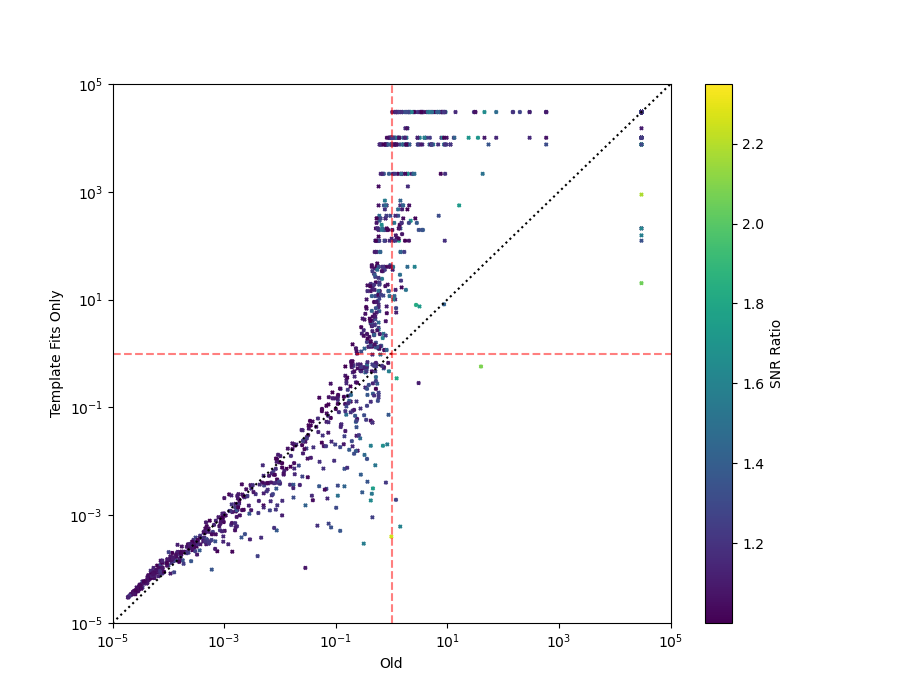
\includegraphics[width=1\textwidth]{images/5_pycbclive/ifar_vs_ifar_snr_ratio_new.png}
  \end{minipage}
  \caption{}
  \label{fig:pycbclive-ifar-ifar-snr-ratio}
\end{figure}
%
It can be seen that there are a number of points in regions of interest (figure~\ref{fig:pycbclive-ifar-ifar-fits-only-0s}) that have been downranked by the new search specifically because they have a high SNR ratio in the old statistic.

\subsection{\label{sec:pycbclive-top-right}Reduced Significance of Previously Highly Significant Injections}

The first region to investigate is the red box in the top-right corner of figure~\ref{fig:pycbclive-ifar-ifar-fits-only-0s}. These are injections that were found with the maximum significance by the old statistic but they have been downranked by the inclusion of template fitting in the ranking statistic. While they have been downranked, they are still all found with a high significance above threshold. 

This region contains $24$ injections, which we can split into two groups for investigation: $12$ injections found with the same trigger in both searches and $12$ injections found with different triggers in both searches. Figure~\ref{fig:pycbclive-top-right-region} shows the distribution of same and different trigger injections in the region, it can be seen that both groups overlap and there isn't a distinct population difference.
%
\begin{figure}
       \centering
    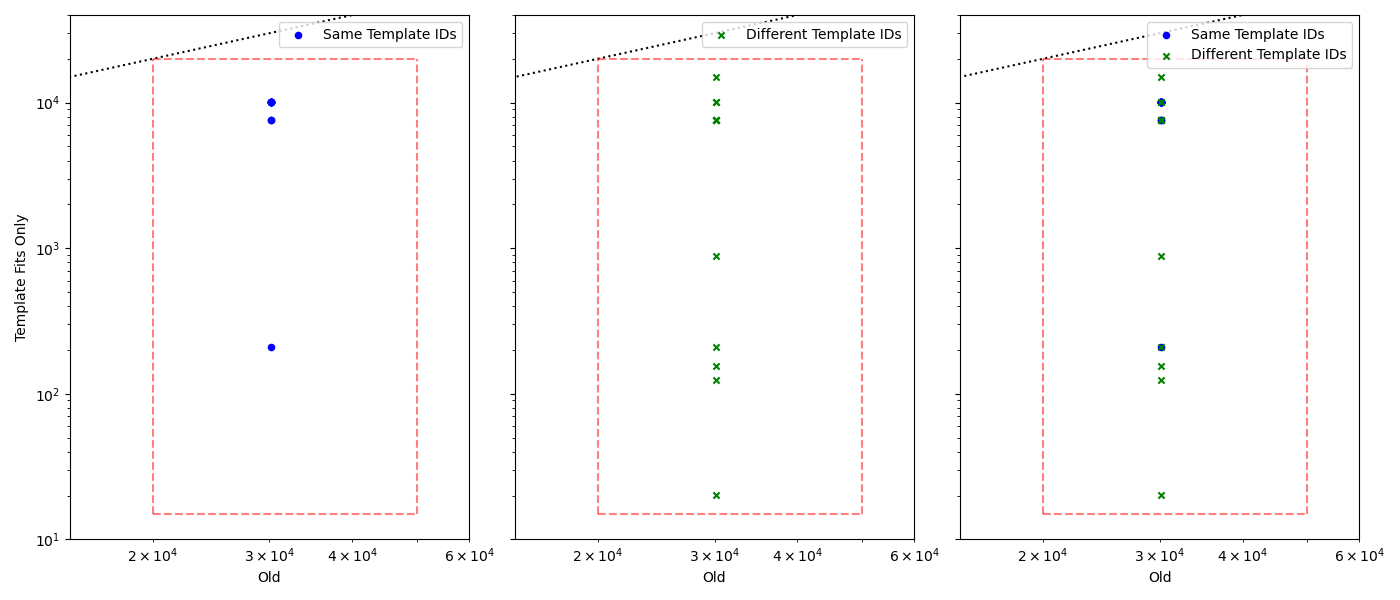
\includegraphics[width=1\textwidth]{images/5_pycbclive/ifar_vs_ifar_subplots.png}
    \caption{}
    \label{fig:pycbclive-top-right-region}
\end{figure}
%
% Same Triggers
When an injection is found with the same trigger across both searches we can dismiss any changes in $\rho_{new}$ being the cause for an IFAR drop and focus solely on the previously discussed changes like poor template fits and noise rate contribution changes.

First we must double check these were found with identical SNR and $\chi^{2}$ values, this was how we discovered the time discrepancy described in section~\ref{sec:pycbclive-diff-start-times}. Table~\ref{tab:pycbclive-same-trigs-snr-chi} shows $5$ of the $12$ injections and their single detector parameters where it can be plainly seen that these are consistent between searches. This is true for the other $7$ injections also.
%
\begin{table}[ht]
    \centering
    % \small
    \setlength{\tabcolsep}{5pt}
    \begin{tabular}{|l|c|c|c|c|c|c|c|c|c|c|c|c|}
        \toprule
        & \multicolumn{6}{c|}{New} & \multicolumn{6}{c|}{Old} \\
        \hline
        & \multicolumn{3}{c|}{H1} & \multicolumn{3}{c|}{L1} & \multicolumn{3}{c|}{H1} & \multicolumn{3}{c|}{L1} \\
        \hline
        \textbf{Inj Idx} & \textbf{SNR} & \textbf{$\chi^{2}$} & \textbf{SG} & \textbf{SNR} & \textbf{$\chi^{2}$} & \textbf{SG} & \textbf{SNR} & \textbf{$\chi^{2}$} & \textbf{SG} & \textbf{SNR} & \textbf{$\chi^{2}$} & \textbf{SG} \\
        \hline
        1 & 1.1 & 2.2 & 3.3 & 4.4 & 5.5 & 6.6 & 1.1 & 2.2 & 3.3 & 4.4 & 5.5 & 6.6 \\
        2 & 1.1 & 2.2 & 3.3 & 4.4 & 5.5 & 6.6 & 1.1 & 2.2 & 3.3 & 4.4 & 5.5 & 6.6 \\
        3 & 1.1 & 2.2 & 3.3 & 4.4 & 5.5 & 6.6 & 1.1 & 2.2 & 3.3 & 4.4 & 5.5 & 6.6 \\
        4 & 1.1 & 2.2 & 3.3 & 4.4 & 5.5 & 6.6 & 1.1 & 2.2 & 3.3 & 4.4 & 5.5 & 6.6 \\
        5 & 1.1 & 2.2 & 3.3 & 4.4 & 5.5 & 6.6 & 1.1 & 2.2 & 3.3 & 4.4 & 5.5 & 6.6 \\
        \bottomrule
    \end{tabular}
    \caption{Sample data with new and old metrics}
    \label{tab:pycbclive-same-trigs-snr-chi}
\end{table}
%
Looking at the template fit parameter values for the triggers themselves is the first step in identifying any `poor' fits. We can look at the $\rho_{new}$, $\alpha$ and $\mu$ values of each of the $12$ same trigger injections and calculate the single detector log noise rate, these values can be seen in table~\ref{tab:pycbclive-top-right-same-trigs-fits}, alongside the combined log noise rate, log signal rate (which is equal in both searches for the same trigger injections) and the ranking statistic value (calculated simply using $R = ln(r_s) - Comb. ln(r_n)$).
%
\begin{table}[ht]
    \centering
    \small
    \setlength{\tabcolsep}{5pt}
    \rowcolors{2}{white}{lightgray}
    \begin{adjustbox}{minipage=\linewidth-0cm, margin=-4cm 0pt 0pt 0cm}
    \begin{tabular}{lccccccccccc}
        \toprule
        & \multicolumn{4}{c}{\textbf{H1}} & \multicolumn{4}{c}{\textbf{L1}} \\
        \cmidrule(lr){2-5} \cmidrule(lr){6-9}
        \textbf{Inj Idx} & \textbf{$\rho_{new}$} & \textbf{$\alpha$} & \textbf{$\mu$} & \textbf{ln(r$_n$)} & \textbf{$\rho_{new}$} & \textbf{$\alpha$} & \textbf{$\mu$} & \textbf{ln(r$_n$)} & \textbf{Comb. ln(r$_n$)} & \textbf{ln(r$_s$)} & \textbf{Rank. Stat.} \\
        \midrule
        8015 & 8.53 & 2.60 & 24.5 & -2.42 & 9.35 & 2.75 & 22.5 & -5.07 & -11.22 & 0.55 & 11.77 \\
        8026 & 9.31 & 2.37 & 9.4 & -4.74 & 8.88 & 2.52 & 14.4 & -3.67 & -12.14 & -0.91 & 11.23 \\
        8110 & 8.99 & 2.37 & 9.4 & -3.97 & 10.30 & 2.52 & 14.4 & -7.26 & -14.96 & -4.78 & 10.18 \\
        9222 & 10.09 & 2.78 & 15.0 & -7.63 & 9.11 & 2.63 & 23.0 & -4.07 & -15.44 & -3.04 & 12.40 \\
        9365 & 7.34 & 2.57 & 24.0 & 0.68 & 10.88 & 2.28 & 29.0 & -6.94 & -9.99 & 0.14 & 10.13 \\
        9777 & 8.33 & 2.57 & 33.75 & -1.51 & 9.30 & 2.78 & 34.25 & -4.63 & -9.86 & 1.91 & 11.77 \\
        10105 & 9.23 & 2.01 & 13.67 & -3.18 & 8.89 & 2.95 & 20.0 & -4.46 & -11.37 & -0.31 & 11.06 \\
        10251 & 9.52 & 2.37 & 9.4 & -5.23 & 10.26 & 2.52 & 14.4 & -7.17 & -16.14 & -10.22 & 5.92 \\
        10979 & 8.31 & 2.01 & 13.67 & -1.33 & 10.23 & 2.95 & 20.0 & -8.41 & -13.47 & -2.02 & 11.45 \\
        11386 & 12.34 & 2.37 & 9.4 & -11.91 & 6.47 & 2.52 & 14.4 & 2.41 & -13.22 & -5.02 & 8.20 \\
        11608 & 9.93 & 1.93 & 14.5 & -4.24 & 7.68 & 2.83 & 23.75 & -0.56 & -8.52 & 1.07 & 9.59 \\
        13845 & 8.40 & 2.37 & 9.4 & -2.57 & 10.37 & 2.52 & 14.4 & -7.44 & -13.74 & -1.53 & 12.21 \\
        \bottomrule
    \end{tabular}
    \end{adjustbox}
    \caption{}
    \label{tab:pycbclive-top-right-same-trigs-fits}
\end{table}
%
To demonstrate how the addition of template fits can cause the downranking of an injections we pick injection $10251$ which had the most significant drop, from maximum IFAR in the old statistic to an IFAR of $209.55$ years when found with the new statistic. We display the ranking statistic components for both searches in tables~\ref{tab:pycbclive-10251-new-stat} and ~\ref{tab:pycbclive-10251-old-stat}.
%
\begin{table}[ht]
    \centering
    \setlength{\tabcolsep}{4pt}
    \begin{minipage}{0.48\textwidth}
        \centering
        \rowcolors{2}{white}{lightgray}
        \begin{adjustbox}{minipage=\linewidth-0cm, margin=0cm 0cm 0cm 0cm}
        \begin{tabular}{lcc}
            \toprule
            \textbf{Inj Idx = 10251} & \textbf{New Trigger} \\
            \midrule
            Comb Log(Noise Rate)  & -16.14 \\
            Log(Signal Rate) & -10.22 \\
            $R_{new}$ & 5.92 \\
            IFAR & 209.55 \\
            \bottomrule
        \end{tabular}
        \end{adjustbox}
        \caption{}
        \label{tab:pycbclive-10251-new-stat}
    \end{minipage}
    \hfill
    \begin{minipage}{0.48\textwidth}
        \centering
        \rowcolors{2}{white}{lightgray}
        \begin{tabular}{lcc}
            \toprule
            \textbf{Inj Idx = 10251} & \textbf{Old Trigger}\\
            \midrule
            $\rho_{H1,new}^2 + \rho_{L1,new}^2$   & 195.90 \\
            Log(Signal Rate) & -10.22 \\
            $R_{new}$ & 13.25 \\
            IFAR & 30174.69 \\
            \bottomrule
        \end{tabular}
        \caption{}
        \label{tab:pycbclive-10251-old-stat}
    \end{minipage}
\end{table}
%
It is important to remember that we cannot directly compare ranking statistic values between the searches, the only value we can compare is the log signal rate which is the same for both searches due to this injection being found with the same trigger in both.

Looking at table~\ref{tab:pycbclive-top-right-same-trigs-fits} for injection $10251$ it has low $\alpha$ values of $2.37$ and $2.52$ and therefore is being heavily downranked by the template fits, having a combined log noise rate of $-16.14$. The signal rate of this injection is also very low when compared to the other injections in the table, this was rescued in the old statistic by large SNR values but the template fits have downranked the significanc of the large SNR values due to this template frequently triggering on noise with a large SNR. We can also see that this template appears $5$ times in this table (injections $8026, 8110, 10251, 111386, 13845$). While the template fits have downranked the significance the injection has still been found far above threshold.

% Different Triggers
For the injections that have been found with different triggers, we have already done an investigation into why these injections were found with different trigger (section~\ref{sec:pycbclive-diff-triggers}) and we can use these injections to demonstrate the findings of that section. We create the same table for the injections found with different template ids, table~\ref{tab:pycbclive-top-right-diff-temp-fits}.
%
\begin{table}[ht]
    \centering
    \small
    \setlength{\tabcolsep}{5pt}
    \rowcolors{2}{white}{lightgray}
    \begin{adjustbox}{minipage=\linewidth-0cm, margin=-3.5cm 0pt 0pt 0cm}
    \begin{tabular}{lccccccccccc}
        \toprule
        & \multicolumn{4}{c}{\textbf{H1}} & \multicolumn{4}{c}{\textbf{L1}} \\
        \cmidrule(lr){2-5} \cmidrule(lr){6-9}
        \textbf{Inj Idx} & \textbf{$\rho_{new}$} & \textbf{$\alpha$} & \textbf{$\mu$} & \textbf{ln(r$_n$)} & \textbf{$\rho_{new}$} & \textbf{$\alpha$} & \textbf{$\mu$} & \textbf{ln(r$_n$)} & \textbf{Comb. ln(r$_n$)} & \textbf{ln(r$_s$)} & \textbf{Rank. Stat.} \\
        \midrule
        8466 & 13.50 & 2.78 & 13.00 & -17.27 & 6.58 & 3.01 & 17.50 & 2.21 & -18.79 & -15.67 & 3.12 \\
        8776 & 6.06 & 2.39 & 25.33 & 3.96 & 12.48 & 2.62 & 26.67 & -12.74 & -12.51 & -0.22 & 12.29 \\
        9040 & 6.20 & 1.93 & 14.50 & 2.95 & 11.01 & 2.83 & 23.75 & -9.99 & -10.77 & -1.30 & 9.47 \\
        9338 & 10.78 & 2.68 & 8.73 & -9.66 & 7.16 & 2.08 & 10.96 & 0.70 & -12.69 & -2.74 & 9.95 \\
        9819 & 7.00 & 1.93 & 14.50 & 1.41 & 11.32 & 2.83 & 23.75 & -10.87 & -13.19 & -1.25 & 11.94 \\
        9859 & 10.39 & 2.58 & 12.86 & -7.83 & 6.61 & 3.69 & 14.57 & 1.74 & -9.81 & -4.62 & 5.19 \\
        10071 & 6.65 & 2.09 & 13.43 & 1.97 & 14.53 & 3.03 & 20.71 & -21.69 & -23.45 & -16.34 & 7.11 \\
        10101 & 10.99 & 2.52 & 18.84 & -8.72 & 7.65 & 3.87 & 17.00 & -2.21 & -14.66 & -6.69 & 7.97 \\
        10134 & 6.55 & 2.60 & 24.50 & 2.72 & 8.76 & 2.75 & 22.50 & -3.46 & -4.47 & 0.09 & 4.56 \\
        10297 & 10.59 & 2.58 & 12.86 & -8.35 & 7.96 & 3.69 & 14.57 & -3.27 & -5.35 & -5.53 & -0.18 \\
        10788 & 9.28 & 2.58 & 12.86 & -4.95 & 8.38 & 3.69 & 14.57 & -4.79 & -13.47 & -0.64 & 12.83 \\
        11505 & 10.78 & 2.78 & 13.00 & -9.71 & 6.67 & 3.01 & 17.50 & 1.95 & -11.48 & -5.97 & 5.51 \\
        \bottomrule
    \end{tabular}
    \end{adjustbox}
    \caption{}
    \label{tab:pycbclive-top-right-diff-temp-fits}
\end{table}
%
These injections have very poor fit parameter values with low $\alpha$ value (especially in H1) and high $\mu$ values. One thing that is very clear, especially when compared to the same trigger table, is that these injections were all found with substantial SNR ratios. These injections and their SNR ratios can be seen in figure~\ref{fig:pycbclive-ifar-ifar-snr-ratio} and this is a clear demonstration of how high SNR ratio triggers are favoured in the old statistic but are unbiased in the new statistic. Overall most injections have been found with high combined log noise rates and signal rates which aren't large enough to compensate.

All the injections investigated are still found significantly and will not be missed in future live searches so there is little to worry about in this particular region of the IFAR vs IFAR parameter space with regards to injections being downranked.

\subsection{\label{sec:pycbclive-bottom-right}Previously Detected Injections That Are Now Below Threshold}

The next region were are investigating contains injections that were found above the IFAR threshold of $1$ year and when using the new statistic have now been found below the IFAR threshold. These are found in the bottom-right quadrant in the blue box in figure~\ref{fig:pycbclive-ifar-ifar-fits-only-0s}, close to the IFAR threshold vertical red dashed line, a close-up is shown in figure~\ref{fig:pycbclive-bottom-right-region}. This region contains 5 injections, we can investigate each of these injections individually to determine the cause of downranking.
%
\begin{figure}
       \centering
    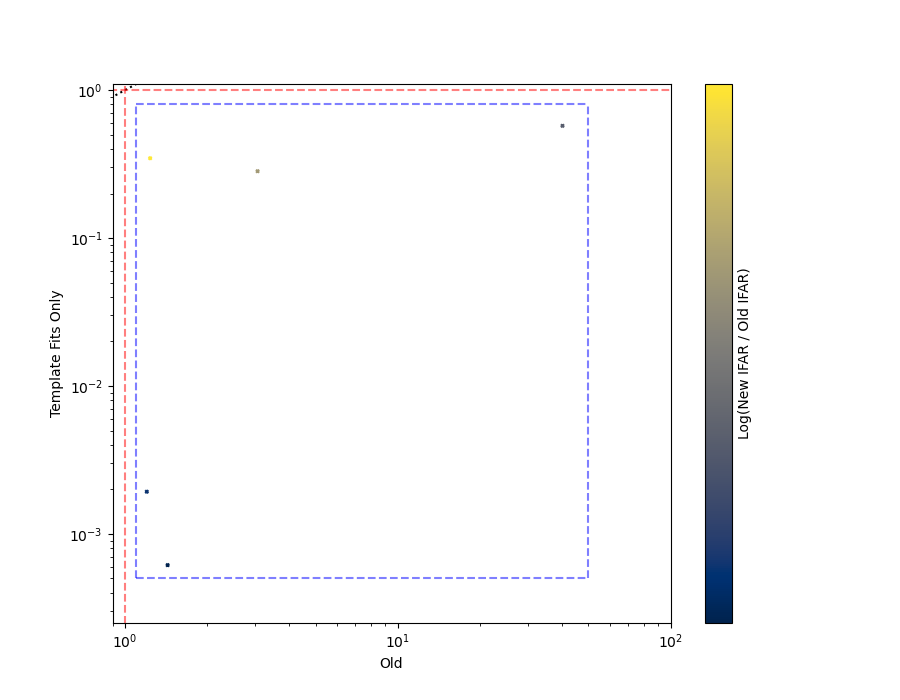
\includegraphics[width=1\textwidth]{images/5_pycbclive/prev_found_ifar_vs_ifar_region.png}
    \caption{}
    \label{fig:pycbclive-bottom-right-region}
\end{figure}
%
We can look at the numerical values associated with each injection, this is shown in table~\ref{tab:pycbclive-bottom-right-rank-stat}.
%
\begin{table}[ht]
    \centering
    \small
    \setlength{\tabcolsep}{4pt}
    \rowcolors{2}{white}{lightgray}
    \begin{adjustbox}{minipage=\linewidth-0cm, margin=-5cm 0pt 0pt 0cm}
    \begin{tabular}{lccccccccccccc}
        \toprule
        & \multicolumn{4}{c}{\textbf{H1}} & \multicolumn{4}{c}{\textbf{L1}} & \multicolumn{3}{c}{\textbf{New}} & \multicolumn{2}{c}{\textbf{Old}} \\
        \cmidrule(lr){2-5} \cmidrule(lr){6-9} \cmidrule(lr){10-12} \cmidrule(lr){13-14}
        \textbf{Inj Idx} & \textbf{$\rho_{new}$} & \textbf{$\alpha$} & \textbf{$\mu$} & \textbf{ln(r$_n$)} & \textbf{$\rho_{new}$} & \textbf{$\alpha$} & \textbf{$\mu$} & \textbf{ln(r$_n$)} & \textbf{Comb. ln(r$_n$)} & \textbf{ln(r$_s$)} & \textbf{IFAR} & \textbf{ln(r$_s$)} & \textbf{IFAR} \\
        \midrule
        8313 & 5.87 & 2.39 & 15.50 & 5.33 & 12.21 & 3.28 & 19.75 & -16.20 & -14.60 & -15.17 & 0.57 & -15.17 & 40.18 \\
        9120 & 7.83 & 2.89 & 12.69 & -1.69 & 4.89 & 4.07 & 16.49 & 11.25 & 5.83 & -3.10 & 0.00062 & -14.96 & 1.43 \\
        10085 & 5.29 & 2.32 & 10.00 & 8.33 & 6.75 & 1.44 & 18.21 & 2.19 & 6.79 & -0.35 & 0.0019 & -16.15 & 1.20 \\
        10256 & 9.57 & 2.71 & 16.16 & -5.92 & 5.30 & 3.77 & 19.30 & 8.95 & -0.69 & -1.65 & 0.35 & -1.65 & 1.24 \\
        10955 & 8.24 & 2.32 & 10.00 & -2.05 & 9.14 & 1.44 & 18.21 & -1.26 & -7.04 & -8.38 & 0.28 & -8.38 & 3.06 \\
        \bottomrule
    \end{tabular}
    \end{adjustbox}
    \caption{}
    \label{tab:pycbclive-bottom-right-rank-stat}
\end{table}
%
These injections demonstrate a few different cases for injection downranking. Injection $8313$ was found with the same trigger in both searches and while the new statistic's combined noise rate is low it isn't enough to overcome the very low signal rate. The 
$\alpha$ values are low and the $\mu$ values are high indicating poor template fits, and $\rho_{new, H1}$ is below $\rho_{thresh}$ and takes an $\alpha$ of $\alpha_{below} = 6.0$ which (when using equation~\ref{eqn:pycbclive-single-log-noise-rate}) has the function of adding a great amount of log noise rate than if the template's $\alpha$ was used.

Injection $9120$ was found with low SNRs in both detectors with $\rho_{new, L1}$ being below $\rho_{thresh}$ which, as seen by the detector \textbf{ln(r$_n$)} columns, contributes massively to the combined log noise rate. This injection was seen with a different trigger in the new search with a higher signal rate but again, not enough to compensate for the noise rate. This is the same for injections $10085$ and $10256$.

Finally, injection $10955$ was found with the same trigger in both searches and is seen with decent SNR in both detectors but the $\alpha$ values are poor, especially in L1. This produces a high combined log noise rate which the signal rate couldn't overcome. These five injections are problematic, being injections that we have observed with the previous statistic and are now missing but we understand why they have been downranked in each case. Missing these injections is a trade-off with observing so many more newly significant injections.

\subsection{\label{sec:pycbclive-bottom-left}Near-Threshold Injections Still Being Missed}

The final region we are investigating is those injections which were marginally missed near the 1 year threshold when searched for using the old statistic, between an IFAR of 0.1 and 1 years, and then were further downranked by including template fitting in the statistic, these can be seen in the bottom-left quadrant's orange box in figure~\ref{fig:pycbclive-ifar-ifar-fits-only-0s}.  This is an important region because these are the signals which are close to the IFAR threshold and we want to recover these with an improved statistic.

This region contains a large number on injections so we need to look at the broad reasons behind the downranking as opposed to the individual injection reasons. The investigation of this region is where we discovered the impact of the SNR ratio in the noise rate contribution (described in section~\ref{sec:pycbclive-diff-triggers}). Our initial hypothesis was poor fits, similar to the other regions.
%
\begin{figure}
    \centering
    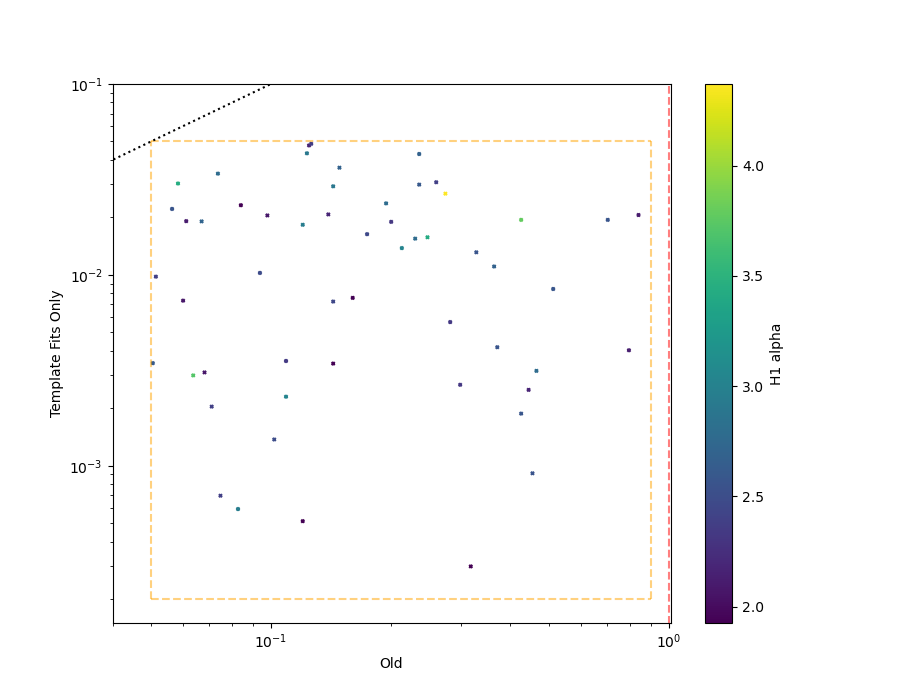
\includegraphics[width=1\textwidth]{images/5_pycbclive/bl_h1_alpha.png}
    \caption{}
    \label{fig:pycbclive-bottom-left-h1-alpha}
\end{figure}
%
\begin{figure}
    \centering
    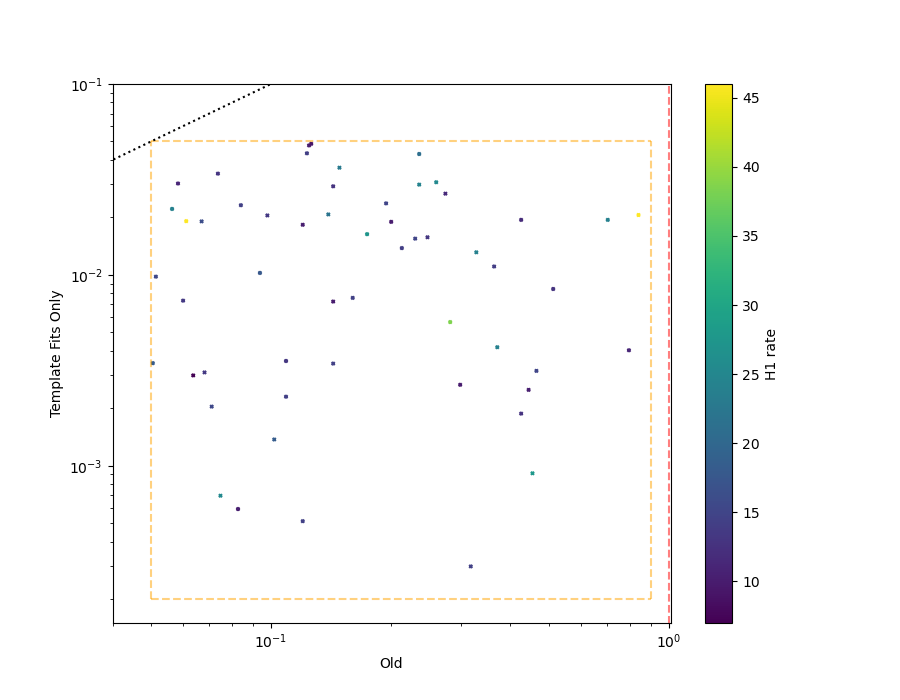
\includegraphics[width=1\textwidth]{images/5_pycbclive/bl_h1_rate.png}
    \caption{}
    \label{fig:pycbclive-bottom-left-h1-rate}
\end{figure}
%
Figures~\ref{fig:pycbclive-bottom-left-h1-alpha} and~\ref{fig:pycbclive-bottom-left-h1-rate} show the IFAR vs IFAR plot for this region with colours representing the H1 $\alpha$ and $\mu$ of each injection. We would hope to see a trend of worse fits the further from the $y=x$ diagonal line we get but the majority of points have low $\alpha$ values with some having high $\alpha$ values. There is a similar story for $\mu$, no clear correlation between $\alpha$ and $\mu$ and injection position in this region.

We can further plot both the single detector H1 log noise rate and the combined log noise rate to see if these are responsible for the downranking, again we would expect to see a higher noise rate the further we are from the diagonal,
%
\begin{figure}
    \centering  
    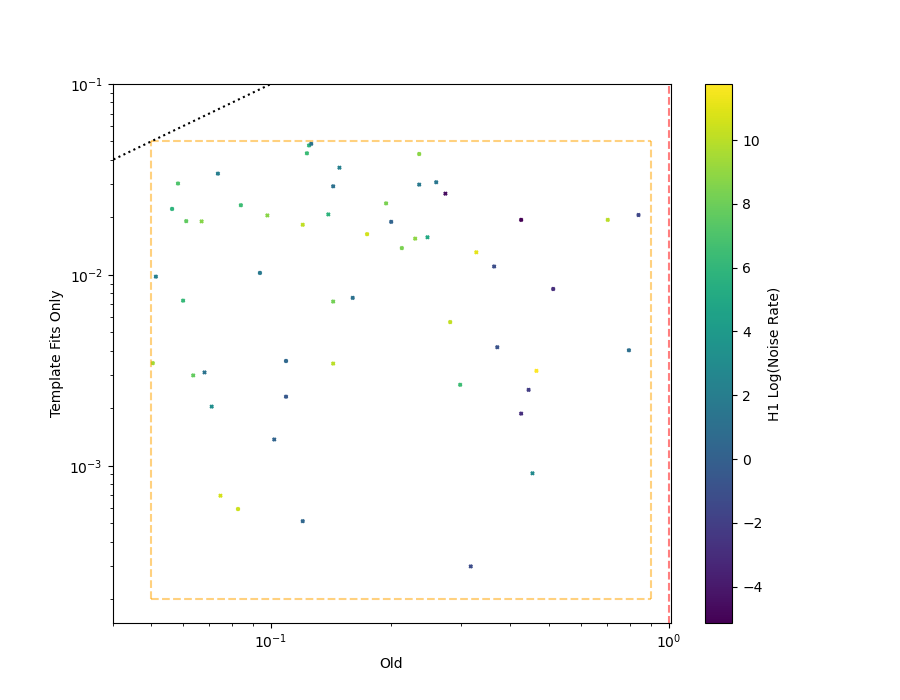
\includegraphics[width=1\textwidth]{images/5_pycbclive/bl_h1_lognoise.png}
    \caption{}
    \label{fig:pycbclive-bottom-left-h1-log-noise-rate}
\end{figure}
%
\begin{figure}
    \centering
    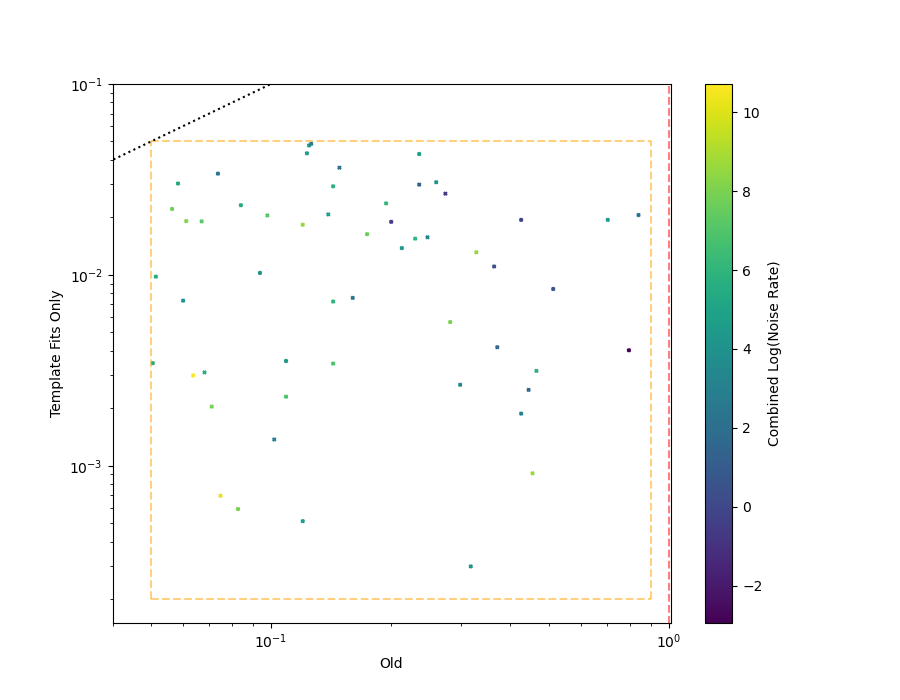
\includegraphics[width=1\textwidth]{images/5_pycbclive/bl_comb_lognoise.png}
    \caption{}
    \label{fig:pycbclive-bottom-left-comb-log-noise-rate}
\end{figure}
%
but from figures~\ref{fig:pycbclive-bottom-left-h1-log-noise-rate} and~\ref{fig:pycbclive-bottom-left-comb-log-noise-rate} we can see that isn't true and in fact some low combined noise rate values for values far from the diagonal. It is at this point we look to the influence of the ranking statistic formulation and more specifically the noise rate contributions, discussed in section~\ref{sec:pycbclive-noise-contrib}. Figure~\ref{fig:pycbclive-bottom-left-snr-ratio} shows the ratio of the two detector $\rho_{new}$ values found by the new statistic (where the ratio is always calculated to be greater than 1)
%
\begin{figure}
  \centering
  \begin{minipage}[t]{1.0\linewidth}
  
    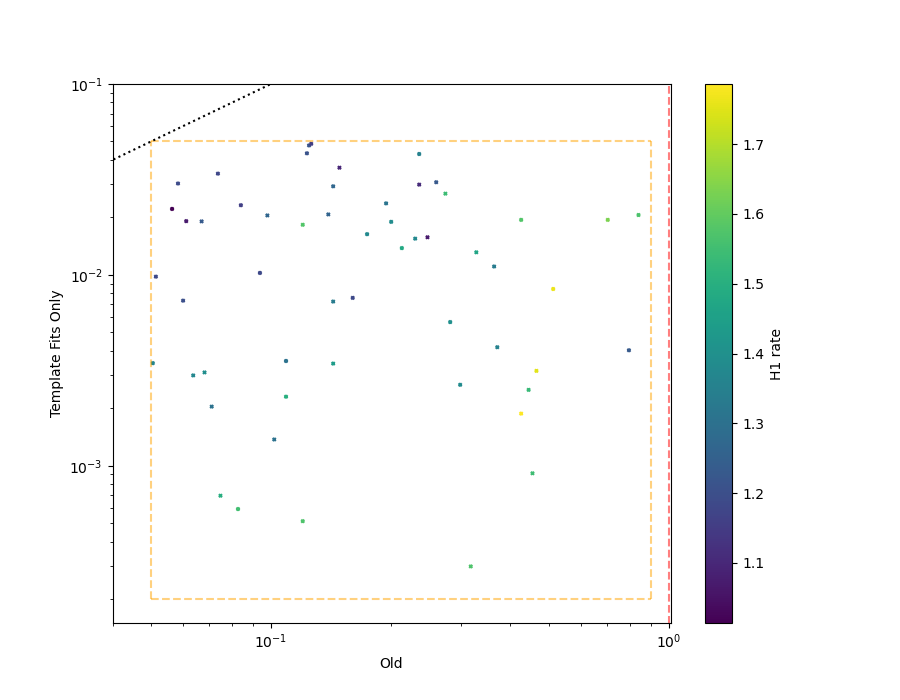
\includegraphics[width=1\textwidth]{images/5_pycbclive/bl_snr_ratio.png}
    \caption{}
    \label{fig:pycbclive-bottom-left-snr-ratio}
  
  \end{minipage}
\end{figure}
%
This figure tells a large part of the story for this region. There is a visible trend that the injections further from the diagonal have a higher SNR ratio, explaining why they have been downranked to a greater extent that other similar injections. What we are seeing is injections found with a much higher $\rho_{new}$ in one detector when compared to the other, and due to the noise rate contributions described in section~\ref{sec:pycbclive-noise-contrib} and the squared sum of the SNRs being used the difference in SNR value didn't matter as much in the old statistic. In the new statistic however, the contribution from the $\rho_{new}$ is weighted by the template fits parameters $\alpha$ and $\mu$ and simply summed to obtain the combined log noise rate, therefore when one detector has observed a low $\rho_{new}$ it is no longer being compensated for by a large $\rho_{new}$ in the other detector, leading to a dramatic decrease in the significance obtain for these injections.

This is a consequence of the ranking statistic formulation difference between the old statistic and the new statistic and is not concerning, primarily because these injections haven't been seen in the old statistic and still are not seen in the new statistic. We are happy that we understand all three of these regions and the overall sensitivity increase of introducing the new statistic to the live search more than compensates for these injections being downranked.

\section{\label{sec:pycbclive-mdc-test}Full Template Bank Test on the Mock Data Challenge Infrastructure}

Finally, we were able to use the PyCBC Live Mock Data Challenge (MDC) testing computational resources to run a full template bank search to test the implementation in an environment that is effectively identical to the actual PyCBC Live search, with the inclusion of the new ranking statistic code. This environment is allocated a number of private nodes equivalent to that of the real PyCBC Live search so we didn't run into the aforementioned memory issues.

We followed the same procedure as done for the offline test, creating template fits across the whole bank for a week of data and then running the search using these template fits on the proceeding weeks. We did not update the fits throughout this test. The purpose of this test was not to test sensitivity improvements, as these have already been tested in offline, it was to test for bugs and if the inclusion of template fits adds any latency to the search. We identified and fixed a number of bugs which were introducing major latency to the search, after fixing there is no latency difference between the current configuration and the new live search configuration.

\section{\label{sec:pycbclive-conclusion}Conclusion}







% TO BE DISCUSSED AS AN ASIDE?
\subsection{\label{sec:pycbclive-diff-start-times}Different Search Start Times}

While investigating these regions we discovered a very important contribution to the IFAR vs IFAR distribution that we hadn't intended to include in our injection sets. 

To take a step back to explain how this problem was introduced into our data and describe how the initial searches were performed. We have two searches: one with the old statistic, one with the new statistic (including any new components). One of the new components is the template fitting statistic and this required that an additional week of search had to be performed using the old statistic, a week prior to the actual search. Therefore for simplicity we ran the old statistic live search over two weeks with no interruptions and the new statistic live search simply over the second week only, after creating the template fitting files.

The old statistic search began at a GPS time of $1262390400$, with the second week beginning at $1262995020$ so the new statistic search began at this time. The problem is that the difference between the week 1 and week 2 start time ($604,620$) is not divisible by $8$, which is our stride time in live. This means that when the old statistic search is crossing the boundary between week 1 and week 2 it will start week 2 on the stride time $1262995024$ which is four seconds after the offical beginning of week 2.

An easy to see problem is that the old statistic search will have had more initial time to bed in the search, so it had knowledge of the $256$ seconds prior to the start of week 2, we account for this and exclude $256$ seconds of data from the start of both searches. This should prevent the old statistic search from reporting seeing more injections than the new statistic.

A bigger problem is that the live searches are analysing different data as they are searching, there is always going to be a $4$ second difference in the data being analysed at any one time. While both searches will search through the same data (except the old statistic will miss the final $4$ seconds of week 2) the PSD for the $256$ seconds of data being analysed can be different in every stride. All the injections have the potential to be seen with a different SNR due to different noise in the data that is being analysed, therefore while the injections might've been seen with the same template, it was not seen with the same trigger which will change the significance of our injections.

This was discovered when we were seeing different SNR and $\chi^{2}$ values for injections with identical trigger templates and times. Aside from computing issues, our searches should be identical and if they are searching the same data with the same template they should always recover the same values from matched filtering, evidently they weren't due to this mismatch in data.

To solve this problem we re-ran the new statistic search but with the start time being equal to the start time of the old statistic search, $1262995024$. With this re-run search we can re-plot figure~\ref{fig:pycbclive-ifar-ifar-fits-only-4s} now that the same data is being analysed in every stride by both searches, this IFAR vs IFAR plot can be seen in figure~\ref{fig:pycbclive-ifar-ifar-fits-only-0s},
%
\begin{figure}
       \centering
    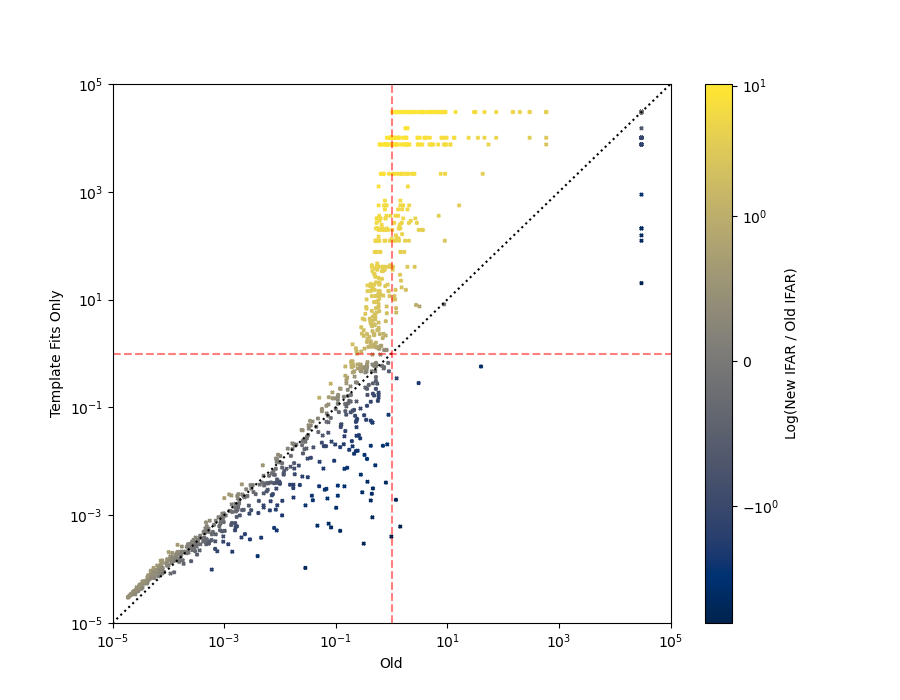
\includegraphics[width=1.2\textwidth]{images/5_pycbclive/fits_only_0s_ifar_vs_ifar_log_ifar_diff.png}
    \caption{}
    \label{fig:pycbclive-ifar-ifar-fits-only-0s}
\end{figure}
%
and you can see this correction has reduced the spread in the distribution of injections dramatically and is accounting for a lot of the random nature the distribution had in the lower-left quadrant. With this new IFAR vs IFAR plot we are able to re-identify the three regions which will be focus the rest of this section discussing, these regions are highlighted in figure~\ref{fig:pycbclive-ifar-ifar-fits-only-0s}.
%
\begin{figure}
    \centering  
    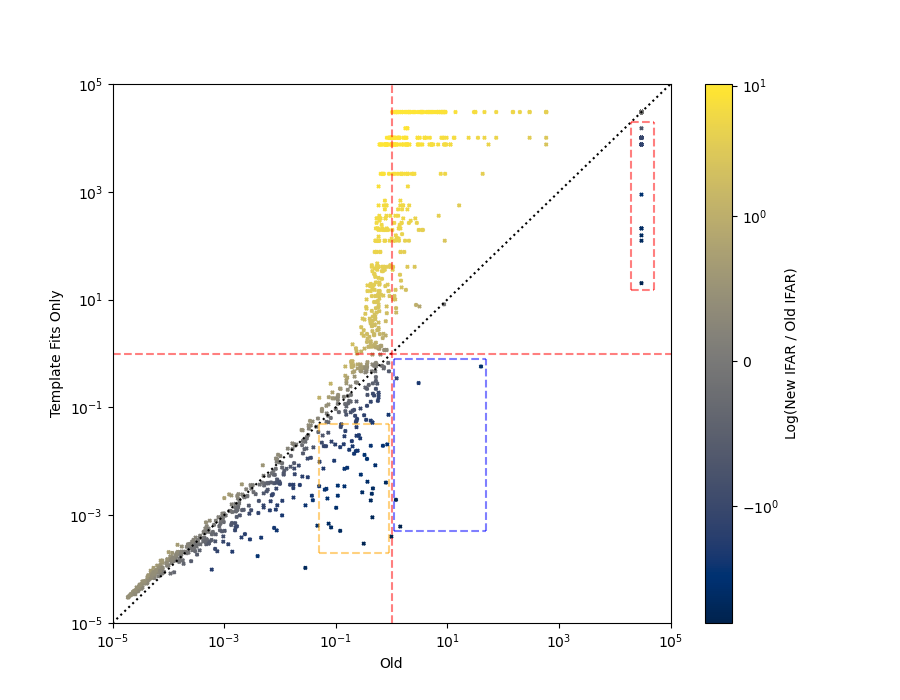
\includegraphics[width=1.2\textwidth]{images/5_pycbclive/fits_only_0s_ifar_vs_ifar_regions.png}
    \caption{}
    \label{fig:pycbclive-ifar-ifar-fits-only-0s-regions}
\end{figure}
%
\begin{figure}
    \centering
    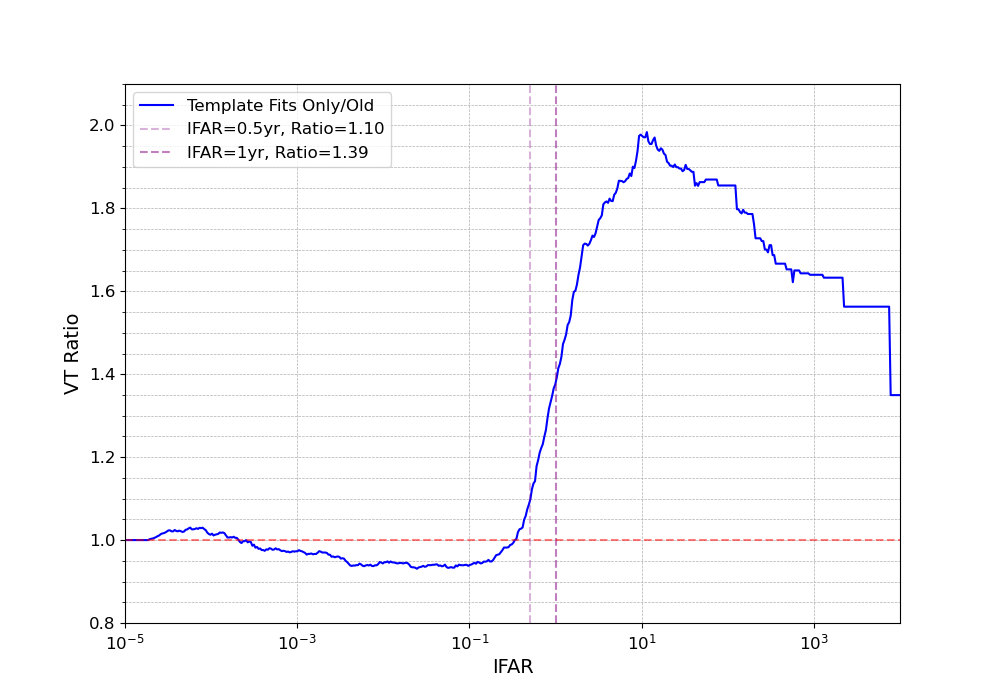
\includegraphics[width=1\textwidth]{images/5_pycbclive/fits_only_0s_vt_ratio.png}
    \caption{}
    \label{fig:pycbclive-sensitivity-fits-only-0s}
\end{figure}
%
Of the $1275$ jointly observed injections: $704$ are seen with a higher IFAR when including template fits, $309$ with a lower IFAR and, $262$ with the same IFAR. This isn't a complete picture, we don't want to see just an increase in the number of injections with a higher IFAR but higher IFAR values for all out injections. To see this we can look at the VT ratio sensitivity plot, shown in figure~\ref{fig:pycbclive-sensitivity-fits-only-0s}.


% ORIGINAL SENSITIVTY
% \begin{figure}
%   \centering
%   \begin{minipage}[t]{1.0\linewidth}
  
%     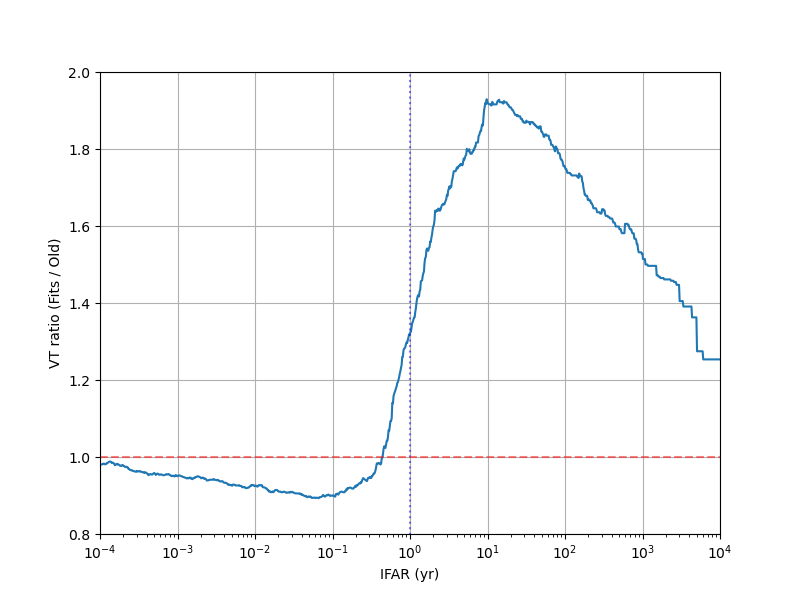
\includegraphics[width=1.0\textwidth]{images/5_pycbclive/ratio.png}
%     \caption{The sensitive volume ratio between the new search and the old search. Calculated by sampling the number of injections found in both searches with an IFAR above the x value and dividing the number in the new search by the number from the old search.}
%     \label{fig:pycbclive-psdvar-4s-sensitivity}

%   \end{minipage}
% \end{figure}
